%%
%% This is file `sample-authordraft.tex',
%% generated with the docstrip utility.
%%
%% The original source files were:
%%
%% samples.dtx  (with options: `authordraft')
%% 
%% IMPORTANT NOTICE:
%% 
%% For the copyright see the source file.
%% 
%% Any modified versions of this file must be renamed
%% with new filenames distinct from sample-authordraft.tex.
%% 
%% For distribution of the original source see the terms
%% for copying and modification in the file samples.dtx.
%% 
%% This generated file may be distributed as long as the
%% original source files, as listed above, are part of the
%% same distribution. (The sources need not necessarily be
%% in the same archive or directory.)
%%
%% The first command in your LaTeX source must be the \documentclass command.
\documentclass[sigconf,anonymous]{acmart}

\usepackage{booktabs}
\usepackage{todonotes}


%%
%% \BibTeX command to typeset BibTeX logo in the docs
\AtBeginDocument{%
  \providecommand\BibTeX{{%
    \normalfont B\kern-0.5em{\scshape i\kern-0.25em b}\kern-0.8em\TeX}}}

%% Rights management information.  This information is sent to you
%% when you complete the rights form.  These commands have SAMPLE
%% values in them; it is your responsibility as an author to replace
%% the commands and values with those provided to you when you
%% complete the rights form.
\setcopyright{acmcopyright}
\copyrightyear{2020}
\acmYear{2020}
\acmDOI{10.1145/1122445.1122456}

%% These commands are for a PROCEEDINGS abstract or paper.
\acmConference[Galway '20]{Galway '20: ACM International Conference on Information and Knowledge Management}{October 19--23, 2020}{Galway, Ireland}
\acmBooktitle{Galway '20: ACM International Conference on Information and Knowledge Management,
  October 19--23, 2020, Galway, Ireland}
\acmPrice{15.00}
\acmISBN{978-1-4503-XXXX-X/18/06}


%%
%% Submission ID.
%% Use this when submitting an article to a sponsored event. You'll
%% receive a unique submission ID from the organizers
%% of the event, and this ID should be used as the parameter to this command.
%%\acmSubmissionID{123-A56-BU3}

%%
%% The majority of ACM publications use numbered citations and
%% references.  The command \citestyle{authoryear} switches to the
%% "author year" style.
%%
%% If you are preparing content for an event
%% sponsored by ACM SIGGRAPH, you must use the "author year" style of
%% citations and references.
%% Uncommenting
%% the next command will enable that style.
%%\citestyle{acmauthoryear}

%%
%% end of the preamble, start of the body of the document source.

\theoremstyle{definition}
\newtheorem{definition}{Definition}[section]
\theoremstyle{hypothesis}
\newtheorem{hypothesis}{Hypothesis}[section]

%\renewcommand{\baselinestretch}{0.98}
\begin{document}

%%
%% The "title" command has an optional parameter,
%% allowing the author to define a "short title" to be used in page headers.
\title{FANG: Leveraging Social Context for Fake News Detection Using Graph Representation}
%Kaz: The following title is more straightforward and better?
%\title{FANG: A Factual News Graph That Leverages Social Context\\ for Fake News Detection}

%%
%% The "author" command and its associated commands are used to define
%% the authors and their affiliations.
%% Of note is the shared affiliation of the first two authors, and the
%% "authornote" and "authornotemark" commands
%% used to denote shared contribution to the research.

\author{Author name}
\email{Email}
\affiliation{
  \institution{Institute}
  \streetaddress{Street}
  \city{City}
  \state{State}
  \postcode{Post code}
}

\author{Author name}
\email{Email}
\affiliation{
  \institution{Institute}
  \streetaddress{Street}
  \city{City}
  \state{State}
  \postcode{Post code}
}

\author{Author name}
\email{Email}
\affiliation{
  \institution{Institute}
  \streetaddress{Street}
  \city{City}
  \state{State}
  \postcode{Post code}
}

\author{Author name}
\email{Email}
\affiliation{
  \institution{Institute}
  \streetaddress{Street}
  \city{City}
  \state{State}
  \postcode{Post code}
}

%%
%% By default, the full list of authors will be used in the page
%% headers. Often, this list is too long, and will overlap
%% other information printed in the page headers. This command allows
%% the author to define a more concise list
%% of authors' names for this purpose.
\renewcommand{\shortauthors}{First-author, et al.}

%%
%% The abstract is a short summary of the work to be presented in the
%% article.
\begin{abstract}

% Min -> @Hoang : incorporate into introduction.  Not abstract material
% The rise of social media and user-generated content has changed how news is shared and consumed online. On the positive side, this has allowed anybody's voice to be heard. On the negative side, it gives rise to disinformation, which has known in the public discourse as ``fake news.''
% The dangers of disinformation became of public concern during the 2016 US Presidential elections, but the current COVID-19 pandemic has taken it to a whole new level, leading to the rise of the first global ``infodemic.''
% There have been a number of manual fact-checking initiatives, but they could not scale due to the tremendous volume and the speed with which fake news propagates. Thus, automatic approaches have been proposed as an alternative.
% This includes \emph{content-based} methods, i.e.,~fact-checking based on existing evidence, and \emph{context-based} methods, which leverage on the public perception of the questionable news. While the former can offer explainable predictions, the latter makes fewer assumptions and takes advantage of the large and readily available wisdom of the crowd. 
% Min: folded this sentence into the abstract later.
% Previous contextual models have focused on performance, but disregarded the importance of representation learning.  
% Min: folded this sentence into the abstract later.
% Here, we show that using enhanced representation of social entities not only improves fake news detection, but also the model's robustness in the case of limited data as well as its applicability to related tasks. 


% Hoang: provide a short background before introducing the framework
%The dangers of disinformation have been of public concern since the 2016 US Presidential elections, but the current COVID-19 pandemic has taken it to a whole new level, leading to the rise of the first global ``infodemic.''
%Amongst automatic fact-checking approaches, \emph{context-based} methods make fewer assumptions than \emph{content-based} methods do, and takes advantage of the large and readily available wisdom of the crowd.
% In particular, we propose Factual News Graph (FANG), a novel graphical social context representation and learning framework, and demonstrate its superiority for capturing context into quality representation over rivaling graphical and non-graphical models. 
We propose Factual News Graph (FANG), a novel graphical social context representation and learning framework for fake news detection. 
Unlike previous contextual models that have targeted performance, our focus is on representation learning.  
Compared to transductive models, FANG is scalable in training as it does not have to maintain all nodes, and is efficient at inference time, without the need to re-process the entire graph.
% Min: Not sure how to add this in.
% FANG is also applicable to related tasks. 
Our experimental results show that FANG is better at capturing social context into a high fidelity representation, compared against recent graphical and non-graphical models. In particular, FANG yields significant improvements in the task of fake news detection, and is robust in the case of limited training data. We further demonstrate that the representations learned by FANG generalize to related tasks, such as predicting the factuality of reporting from a news medium. 
\end{abstract}

%%
%% The code below is generated by the tool at http://dl.acm.org/ccs.cfm.
%% Please copy and paste the code instead of the example below.
%%

\begin{CCSXML}
<ccs2012>
<concept>
<concept_id>10010147.10010178.10010179</concept_id>
<concept_desc>Computing methodologies~Natural language processing</concept_desc>
<concept_significance>300</concept_significance>
</concept>
<concept>
<concept_id>10010520.10010521.10010542.10010294</concept_id>
<concept_desc>Computer systems organization~Neural networks</concept_desc>
<concept_significance>300</concept_significance>
</concept>
<concept>
<concept_id>10002951.10003260.10003282.10003292</concept_id>
<concept_desc>Information systems~Social networks</concept_desc>
<concept_significance>300</concept_significance>
</concept>
<concept>
<concept_id>10003752.10010070.10010071.10010289</concept_id>
<concept_desc>Theory of computation~Semi-supervised learning</concept_desc>
<concept_significance>300</concept_significance>
</concept>
</ccs2012>
\end{CCSXML}

\ccsdesc[300]{Computing methodologies~Natural language processing}
\ccsdesc[300]{Computer systems organization~Neural networks}
\ccsdesc[300]{Information systems~Social networks}
\ccsdesc[300]{Theory of computation~Semi-supervised learning}
%%
%% Keywords. The author(s) should pick words that accurately describe
%% the work being presented. Separate the keywords with commas.
\keywords{Disinformation, Fake News, Social Networks, Graph Neural Networks, Representation Learning}

%%
%% This command processes the author and affiliation and title
%% information and builds the first part of the formatted document.
\maketitle

\section{Introduction}\label{sec:introduction}

\begin{table*}[tbh]
%Kaz: Fixed the position of the caption. In ACM template, we usually put the caption for table at the top while it is at the bottom ACL- or AI-related conferences. It is fine to put the captions for figures at the bottom!
\caption{Engagement of social media users with respect to fake and real news articles. Column 2 shows the time since publication, and columns 4--7 show the distribution of stances  %: S stands for Support, D for Deny, C for Comment, and R for Report.
(S: Support, D: Deny, C: Comment, and R: Report).
}
  \label{table:temporal_engagement}
  \centering
  \small
  \begin{tabular}{p{4cm}ccccccp{6.5cm}}
    \toprule
    \bf News title \textbf{(Label)} & \bf Time & \bf \# Posts & \bf S & \bf D & \bf C & \bf R & \bf Noticeable responses \\ 
    \midrule
  Virginia Republican Wants Schools To Check Children's Genitals & 3h & 38 & .00 & .03 & .19 & .78 & ``DISGUSED SO TRASNPHOBIC'', ``FOR GODS SAKE  GET REAL GOP'', ``You cant make this up folks'' \\ \cline{2-8}
  Before Using Bathroom \textbf{(Fake)}  & 3h - 6h & 21  & .00 & .10 & .1 & .80 & ``Ok This cant be real'', ``WTF IS THIS BS'', ``Rediculous RT'' \\ \cline{2-8}
  & 6h+ & 31 & .00 & .10 & .14 & .76 & ``Cant make this shit up'', ``how is this real'', ``small government'', ``GOP Cray Cray  Occupy Democrats'' \\ \hline
  1,100,000 people have been killed by & 3h & 9 & .56 & .00 & .00 & .44 & ``\#StopGunViolence'', ``guns r the problem'' \\ \cline{2-8}
  guns in the U.S.A. since John Lennon was shot and killed on December 8, 1980 \textbf{(Real)} & 3h+ & 36 & .50 & .00 & .11 & .39 & ``Some 1.15 million people have been killed by firearms in the United States since Lennon was gunned down'', ``\#StopGunViolence'' \\ 
  \bottomrule
  \end{tabular}
\end{table*}

% \begin{table*}[tbh]
% %Kaz: Fixed the position of the caption. In ACM template, we usually put the caption for table at the top while it is at the bottom ACL- or AI-related conferences. It is fine to put the captions for figures at the bottom!
% \caption{Engagement of social users with respect to fake and real articles by the distributions of stances (column 4 to 8 - S: Support, D: Deny, NeuC: Neutral Comment, NegC: Negative Comment, R: Report) over time since publication (column 2).}
%   \label{table:temporal_engagement}
%   \centering
%   \small
%   \begin{tabular}{p{4cm}cccccccp{6.5cm}}
%     \toprule
%     \bf News Title \textbf{(Label)} & \bf Time & \bf \# tweets & \bf S & \bf D & \bf NeuC & \bf NegC & \bf R & \bf Noticeable Responses \\ 
%     \midrule
%   Virginia Republican Wants Schools To Check Children's Genitals & 3h & 38 & .00 & .03 & .03 & .16 & .78 & "DISGUSED SO TRASNPHOBIC", "FOR GODS SAKE  GET REAL GOP", "You cant make this up folks" \\ \cline{2-9}
%   Before Using Bathroom \textbf{(Fake)}  & 3h - 6h & 21  & .00 & .10 & .05 & .05 & .80 & "Ok This cant be real", "WTF IS THIS BS", "Rediculous RT" \\ \cline{2-9}
%   & 6h+ & 31 & .00 & .10 & .07 & .07 & .76 & "Cant make this shit up", "how is this real", "small government", "GOP Cray Cray  Occupy Democrats" \\ \hline
%   1,100,000 people have been killed by & 3h & 9 & .56 & .00 & .00 & .00 & .44 & "\#StopGunViolence", "guns r the problem" \\ \cline{2-9}
%   guns in the U.S.A. since John Lennon was shot and killed on December 8, 1980 \textbf{(Real)} & 3h+ & 36 & .50 & .00 & .11 & .00 & .39 & "Some 1.15 million people have been killed by firearms in the United States since Lennon was gunned down", "\#StopGunViolence" \\ 
%   \bottomrule
%   \end{tabular}
% \end{table*}

Social media have emerged as an important source of information for many people worldwide. Unfortunately, not all such information is true, and some is even malicious. 
%Yet, the astonishing speed with which information spreads in social media poses a challenge to any large-scale information verification effort. 
% According to MIT research~\cite{vosoughi2018spread}, 
% falsehood reaches 1,500 people 6 times faster than true stories, and is 70 times more likely to be retweeted. 
In critical events such as political elections or a pandemic outbreak, disinformation with malicious intent~\cite{shu2017fake}, commonly known as ``fake news'', can disturb social behavior, public fairness, and rationality. During the fight against COVID-19, the WHO addressed the \textit{infodemic} caused by the life-costing fake news related to infections and cures~\cite{thomas_2020}. 
% Pizzagate conspiracy theory\footnote{\scriptsize{\url{https://en.wikipedia.org/wiki/Pizzagate_conspiracy_theory}}}, although debunked later, went viral during the 2016 United States presidential election, wrongfully tarnished the reputation of some candidates and benefited others. 
% The popularity of the term ``fake news'' gave itself the title ``word of the year'' by American Dialect Society\footnote{\scriptsize{\url{https://time.com/5091268/fake-news-word-of-the-year/}}}.
% Fake news detection is a non-trivial task. Although the general public is confident in its ability to discriminate false information, recent studies have shown the opposite results. More specifically, 39\% of Americans claim to be ``very confident'' and an extra 45\% to be ``somewhat confident'' in recognizing fake news, however, 75\% of them view a false story as accurate despite having seen it~\cite{edkins_2016}. 
% % Another study conducted in Singapore shows that 90\% of the subjects falsely believe in at least one out of five fake headlines, even though four out of five Singaporeans claim that they can confidently recognizing fake news~\cite{ng_2018}. 
% As the intention behind fake news is to mislead readers, 
% it is challenging to infer news veracity solely based on its content~\cite{shu2017fake}. 

Many sites and social media have devoted efforts to identify disinformation. For example, Facebook encourages users to report non-credible posts\footnote{\scriptsize{\url{https://www.facebook.com/help/572838089565953?helpref=faq_content}}} and employs professional fact-checkers to expose questionable news. This approach is also used by fact-checking websites such as Snopes,\footnote{\scriptsize{\url{http://snopes.com}}} FactCheck,\footnote{\url{http://www.factcheck.org}} and PolitiFact.\footnote{\scriptsize{\url{http://politifact.com}}} In order to scale with the increasing amount of information, automated news verification systems consider external knowledge databases as evidence~\cite{hassan2017claimbuster,thorne2017extensible,popat2018credeye,augenstein-etal-2019-multifc}. Evidence-based approaches achieve high accuracy and offer potential explainability, but they also take considerable human effort.
% Hoang: gave example for different modalities.
% Min: not clear what you mean by different ``modalities'' here.
Moreover, fact-checking approaches for textual claims based on textual evidences are not easily applicable to claims about images or videos.

Recent research has taken another turn and explored contextual features of the news dissemination process. It has been shown that there are distinctive engagement patterns when social users face fake versus factual news~\cite{ma2016detecting,jin2016news}.
For example, the fake news shown in Table~\ref{table:temporal_engagement} had many engagements shortly after its publication. These are mainly verbatim 
% Hoang: works for me
% Min: word choice? can sub re-circulation for report?
% reports 
re-circulations of the original post, 
explained by the typically appalling content of fake news. After that short time window, we see denial 
% Min GLOBAL BUG: use generic posts, instead of Twitter-specific term `tweets'
posts questioning the validity of the news, and the stance distribution stabilizes afterwards with virtually no support. In contrast, the real news example in Table~\ref{table:temporal_engagement} invokes moderate engagement, mainly comprised of supportive posts that stabilize quickly. Such temporal shifts in user perception serve as important signals for distinguishing fake from real news. 

Previous research proposed partial representations of social context with (\emph{i})~news, sources and users as major entities, and (\emph{ii})~stances, friendship, and publication as major interactions~\cite{jin2014news,popat2017truth,shu2019beyond,popat2016credibility}. However, there was insufficient emphasis on the quality of representation, limited modeling of entities and their interactions, and little focus on minimally supervised settings. 

Naturally, the social context of news dissemination can be represented as a heterogeneous network where nodes are the social entities and the edges represent the interactions between them. Network representations have several advantages over some existing Euclidean-based methods~\cite{ruchansky2017csi,liu2018early} in terms of structural modeling capability for several phenomena such as
% Hoang: changed to "echo chambers" for consistency
% Min: `clusters' over `bubbles'
% bubbles 
echo chambers of users or polarized networks of news media. Graphical models also allow entities to exchange information, via (\emph{i})~homogeneous edges, \textit{i.e.},~user--user relationship, source--source citations, (\emph{ii})~heterogeneous edges, \textit{i.e.},~user--news stance expression, source--news publication, as well as (\emph{iii})~high-order proximity (textit{i.e.},~between users who consistently support or deny certain sources, as illustrated in Figure~\ref{fig:social_graph}). This allows the representation of heterogeneous entities to be dependent, leveraging not only fake news detection, but also related social analysis tasks such as malicious user detection~\cite{SeminarUsers2017} and source factuality prediction \cite{baly2018predicting}.

% Previous works to learn such structure have employed spectral-based approaches ~\cite{shu2019beyond,gupta2012evaluating}, whose expensive matrix factorization (MF) does not account for higher order proximity, and whose representations are highly specific to the discussed task. Furthermore, there has been no in-depth analysis of the learned embeddings and their generalization to related tasks. As correlation to underlying communities, or whether the approach is feasible given a limited annotated news for supervised learning.


% \todo{It is not clear what the columns of Table 1 show. The columns need to be explained in the table caption.}

% Min BUG: this paragraph and then the itemized list seem repetitive.  Can you drop one form instead of having both?
% Hoang: Remove the paragraph
% Here, we propose the Factual News Graph (FANG), a graph learning framework that covers various social entities and the interactions between them, as shown in Figure~\ref{fig:social_graph}, with an emphasis on the temporal stance of social users with respect to questionable news. FANG is based on enhanced representation learning that models both stance and social structure. 
% Unlike previous contextual models, which have targeted performance, here our main focus is on representation learning.  
% % Min BUG: repetitive against the below and the item.  Excise one mention.
% Compared to transductive models, FANG is scalable in its training  as it does not have to maintain all nodes, and it is also efficient at inference time, without the need to re-process the entire graph. FANG is also highly explainable thanks to the attention mechanism of its recurrent aggregator. 

Our main contributions can be summarized as follows:
\begin{enumerate}
    \item We propose a novel graph representation that models all major social actors and their interactions (Figure~\ref{fig:social_graph}). 
    \item We propose the Factual News Graph (FANG), an inductive graph learning framework that effectively captures social structure and engagement pattern, thus improving representation quality.
    % Hoang: fixed
    % Min: see above BUG.  
    % The transductive model is scalable in its training as it does not have to maintain all nodes, and it is efficient at inference time as it does not need to re-process the entire graph.
    \item We report sizeable improvements when using FANG for the task of fake news detection, and we further show that the model is robust in the case of limited training data.
    \item We show that the representations learned by FANG generalize to related tasks such as predicting the factuality of reporting of a news medium.
    \item We demonstrate FANG's explainability thanks to the attention mechanism of its recurrent aggregator.
\end{enumerate}

\begin{figure}[t]
\centering
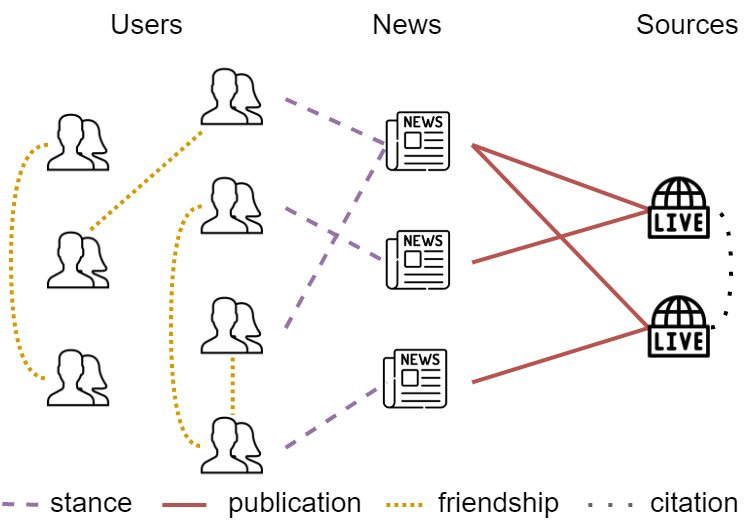
\includegraphics[scale=0.25]{fang_graph.png}
\caption{Graph representation of social context.}
% Hoang: improved graph resolution
% Min: use textured lines to differentiate (dotted, dashed) as well as color, so that users on b/w can see appropriately.  Consider putting the legend below the graph in a 2x2 matrix so that the graph itself can be at a larger resolution if there is space.
% Min: BUG consider cross referencing text in Sect 3.  See comment search for XREF1
\label{fig:social_graph}
\end{figure}

%Kaz: I divided this section into two subsections to make the structure of the paper better. Please check whether the subtitles are relevant or not. 
\section{Related Work}\label{sec:related}
% \begin{table*}[t]
%   \centering
%   \small
% \caption{Comparison between representation learning frameworks of social context}
%   \begin{tabular}{p{2.5cm}|p{4cm}|p{2.5cm}|p{1.25cm}|p{3cm}|p{1.75cm}}
%   \hline
%     Approach & Category & Modeled social entities \& interactions & Temporality & Learning Framework & Structural Expressiveness \\ \hline \cite{castillo2011information,ma2015detect,yang2012automatic} & Feature-based model & 1., 2. & No & Euclidean-based learning & No \\
%     \cite{ruchansky2017csi} & Graph representation \& Euclidean learning & 1., 2., 4., 5. & Yes & MF, RNN & No \\
%     \cite{shu2019beyond} & End-to-end Graph & 1., 2., 3., 4., 5., 6 & No & MF & No \\
%     \cite{kulkarni2018multi} & Graph representation \& Euclidean learning & 2., 3., 6., 7. & No & GNN, Deep Network  & No \\
%     Monti (2019)~\cite{monti2019fake} & End-to-end Graph & 1., 2., 4., 5. & No & GNN & No \\
%     \cite{yuan2019jointly} & End-to-end Graph & 1., 2., 5. & No & GNN, Multi-head attention & No \\ \hline
%     FANG (this work) & End-to-end Graph (supervised), Graph representation \& Euclidean learning (unsupervised) & 1., 2., 3., 4., 5., 6., 7. & Yes & GNN & Yes \\ \hline
%   \end{tabular}
%   \label{table:literature_review1}
% \end{table*}

%Kaz: Highlighted "FANG" with bold fonts
\begin{table*}[tbh]
  \centering
  \small
%\caption{Comparison between representation learning frameworks of social context.}
%Kaz: Rewrite the caption to clearly show what the number denotes. 
\caption{Comparison between representation learning frameworks for social entities (1. users, 2. news, 3. sources) and interactions (4. user-user friendship, 5. user--news engagement, 6. source--news publication, 7. source--source citation).}
  \begin{tabular}{ccccccc}
  \toprule
    \bf Approach & \bf Social entities \& interactions & \bf Temporal & \bf Graphical & \bf Deep & \bf Inductive & \bf Representative \\ 
    \midrule 
    Feature engineering~\cite{castillo2011information,ma2015detect,yang2012automatic} & 1., 2. & & & & \checkmark & \\
    Popat~\cite{popat2017truth,popat2016credibility} & 1., 3., 6. & \checkmark & \checkmark & \checkmark & & \\
    CSI~\cite{ruchansky2017csi} & 1., 2., 4., 5. & \checkmark & \checkmark & & \checkmark & \\
    TriFN~\cite{shu2019beyond} & 1., 2., 3., 4., 5., 6 & & \checkmark & & & \checkmark \\
    MVDAM~\cite{kulkarni2018multi} & 2., 3., 6., 7. & & \checkmark & \checkmark & & \\
    Monti~\cite{monti2019fake} & 1., 2., 4., 5. & \checkmark & \checkmark & & & \\
    GLAN~\cite{yuan2019jointly} & 1., 2., 5. & & \checkmark & \checkmark & & \\ \hline
    \textbf{FANG} \tiny{(Our proposed approach)} & 1., 2., 3., 4., 5., 6., 7. & \checkmark & \checkmark & \checkmark & \checkmark & \checkmark \\ 
    \bottomrule
  \end{tabular}
  \label{table:literature_review}
\end{table*}

%Kaz: The following paragraph may be no need.
%Hoang: I intended this to be a navigation paragraph to improve coherence. We can omit this if space contrained.
In this section, we first review the existing work on contextual fake news detection and the way the social context of news is represented in such work. We then detail recent advances in the Graph Neural Network (GNN) formalism, forming the premise of our proposed graph learning framework. \\

\noindent\textbf{Contextual Fake News detection.}
Previous work on contextual fake news detection can be categorized based on the approach they used to represent and learn the social context. 

Specifically, \emph{Euclidean approaches} represent the social context as a flat vector or as a matrix of real numbers. 
These methods typically learn a Euclidean transformation of the social entity features that best approximates the fake news prediction. The complexity of such transformation varies from the traditional shallow (as opposed to ``deep'') models, \textit{i.e.},~Random Forest or Support Vector Machines (SVM)~\cite{castillo2011information,yang2012automatic} to deep neural networks such as Long Short-Term Memory (LSTM)~\cite{lstm1997hochreiter} that model engagement temporality~\cite{ruchansky2017csi}. However, given our formulation of social context as a heterogeneous network, Euclidean representations are less expressive~\cite{bronstein2017geometric}. Although pioneering work used user attributes such as demographics, news preferences, and social features such as the number of follower and friends~\cite{ma2015detect,shu2017fake}, they do not capture the user interaction landscape \textit{i.e.},~what kind of social figures they follow, which news topics they favor or oppose, etc. Moreover, in graphical representation, node variables are no longer restrained by the independent and identically distributed assumption, and thus reinforce each other's representation via edge interactions.

% Min: is non-Euclidean meant as another name for network-oriented approaches? 
Having acknowledged the above limitations, research has started exploring non-Euclidean or \emph{geometric approaches}.
% Networks in which nodes constantly exchange and propagate information such as trust~\cite{kamvar2003eigentrust} or any auxiliary attributes~\cite{liao2018attributed} have been widely discussed. 
Such work generalized the idea of using social context by modeling an underlying user or the news source network, and developing representations that capture structural features about the entity. The \emph{Capture, Score, and Integrate} (CSI) model~\cite{ruchansky2017csi} used linear dimensionality reduction on user co-sharing adjacency matrix and combined it with news engagement features obtained from a recurrent neural network (RNN). The \emph{Tri-Relationship Fake News} (TriFN) detection framework~\cite{shu2019beyond}, although similar to our approach, neither differentiated user engagements in terms of stance and temporal patterns, nor modeled source--source citations. Furthermore, matrix decomposition approaches, including CSI~\cite{ruchansky2017csi}, can be expensive in terms of graph node counts and ineffective for modeling high-order proximity. 

Other work on citation source network~\cite{kulkarni2018multi}, propagation network~\cite{monti2019fake}, and rumor detection~\cite{yuan2019jointly} used recent advances in GNNs and multi-head attention to learn both local and global structural representations. 
% Hoang: rewrite the following sentence
% Despite the incremental performance improvement in fake news detection, the authors neither considered a comprehensive social context graph nor examined the representation learning of social entities in a minimally supervised setting.
These models are optimized on the sole objective of fake news detection without an emphasis on representation quality.
% Hoang: pointed forward the discussion
% Min: how can you substantiate this claim?  By your results (then point forward to your section)?  Or cited work?  
As a result, they are less robust when presented with limited training data and they generalize poorly to other downstream tasks (see Section~\ref{sec:discussion} below). 
%%%%%
Table~\ref{table:literature_review} offers a summary comparison between the above-described approaches.\\
%Kaz: The following should be specified as the caption at Table 1. So I moved the following sentence to Table 1. 
%The social entities and social interactions are (1) users, (2) news, (3) sources, (4) user--user friendship, (5) user--news engagement, (6) source--news publication, (7) source--source citation. 

%Kaz: I'm not sure the following sub-title is relevant or not. Please improve if you have better idea. In addition, we can skip the following sentence as we have already described it at the beginning of Sec 2.  


\begin{table*}[tbh]
  \centering
  \small
  \caption{Interactions in the social context.}
  \begin{tabular}{llllc}
  \toprule
    \bf Interaction & \bf Linking Entities & \bf Linking Type & \bf Description & \bf Temporal \\ 
    \midrule
    Followership & User-user & Unweighted, undirected & Whether a user follows another user on social media & No \\
    Citation & Source-source & Unweighted, undirected & Whether sources refers to another source via a hyperlink & No \\
    Publication & Source-news & Unweighted, undirected & Whether the source published the target news & Yes \\
    Stance & User-news & Multi-label, undirected & The stance of the user with respect to the news & Yes \\ 
    \bottomrule
  \end{tabular}
  \label{table:social_interactions}
\end{table*}


\noindent\textbf{Graph Neural Network.}
%We also review the recent advancements in GNN, which are at the core our proposed framework. 
GNNs have successfully generalized deep learning methods to model complex relationships and inter-dependencies on graphs and manifolds. A Graph Convolutional Network (GCN) is one of the first methods that effectively approximates convolutional filters~\cite{kipf2016semi}. However, spectral-based GCNs impose a substantial memory footprint in storing the entire adjacency matrix.  They are also not easily adaptable to our heterogeneous graph setting, where nodes and edges of different labels have different information propagation patterns. Furthermore, GCNs do not guarantee  generalizable representations, and they are transductive, requiring the inferred nodes to be present at training time. This is especially challenging for contextual fake new detection or for general social network analysis, as their structure is constantly evolving. 
% Min: Hoang, you seem to be hinting that a dynamic algorithm that can create nodes and edges during inference time is necessary.  IS that what you mean and if so, then you should be more explicit in your following paragraph below.

With all these caveats in mind, we build the present work on GraphSage that generates embeddings by sampling and aggregating features from a node's local neighborhood~\cite{Hamilton2017InductiveRL}. GraphSage offers great flexibility in defining the information propagation pattern with parameterized random walks and recurrent aggregators. It is highly suitable for representation learning with unsupervised node proximity loss, and
% Hoang: I have changed word quality into "generalizable"
% Min: I still am not sure what qualifies as ``quality representation''.  Do you need to be more careful about how you define this meaning?
good generalization in minimal supervision settings. Furthermore, GraphSage is a dynamic inductive algorithm that allows the creation of unseen nodes and edges at inference time.

\section{Methodology}

In this section, we first introduce the notation that we will be using throughout the rest of the paper, and then we formally define the problem of fake news detection. Afterwards, we discuss our methodology, namely the process of construction of our social context graph, the Factual News Graph (FANG), as well as its of its
% Min: Word choice ``rationale'' subbed for original ``rationality''.
underlying rationale. 
Finally, we describe the process of feature extraction from social entities as well as the modeling of their interactions. 

\subsection{Fake News Detection Using Social Context}
In order to ensure a consistent representation, let us first define the social context $C$ with 
% Min: refactor out `Let'
% its entities and interactions:
its entities and interactions, as shown in Figure~\ref{fig:social_graph}:
\begin{enumerate}
% Min: would be good to cross reference this to entities in Fig. 1 by labeling those entities and edges.  Label XREF1.
%    \item Let 
    \item $A=\{a_1, a_2,...\}$ is the list of questionable \textbf{news articles}, where each $a$ is modeled as a feature vector $\boldsymbol{x}_{a}$.
%    \item Let 
    \item $S=\{s_1, s_2,...\}$ is the list of \textbf{news sources}, where each source $s_j$ has published at least one article in $A$, and each $s$ is modeled as a feature vector $\boldsymbol{x}_{s}$.
%    \item Let 
% Min: pop a line.  Edited down
%    \item $U=\{u_1, u_2,...\}$ be the list of \textbf{social users}, where each user has engaged in spreading any article in $A$ or has a connection with any user in $U$, where each $u$ is modeled as a feature vector $\boldsymbol{x}_{u}$.
    \item $U=\{u_1, u_2,...\}$ is the list of \textbf{social users}, where each social user has engaged in spreading an article in $A$ or is connected with another social user, where each $u$ is modeled as a feature vector $\boldsymbol{x}_{u}$.
%    \item Let 
    \item $E=\{e_1, e_2,...\}$ is the list of
    % Min: need \bf?
%    interactions, where each interaction $e=\{v_1, v_2, t, x_e\}$ is a relation between two entities $v_1, v_2\in A\cap S\cap U$ at time $t$, where $t$ can be absent in interactions that are time-insensitive. The interaction type of $e$ is defined as the label $x_{e}$.
    {\bf interactions}, where each interaction $e=\{v_1, v_2, t, x_e\}$ is a relation between two entities $v_1, v_2\in A\cap S\cap U$ at time $t$, where $t$ can be absent in interactions that are time-insensitive. The interaction type of $e$ is defined as the label $x_{e}$.
\end{enumerate}

Table~\ref{table:social_interactions} summarizes the characteristics of different types of interactions, both homogeneous and heterogeneous. 
%Kaz: Here, only Fig 1 is fine to refer to.  
%and Figure~\ref{fig:fang_overview}.
% Hoang: We gave the examples in Table 1 highlighting the importance of temporality. I will refer to it again.
% Min: this temporality point deserves more emphasis in the introduction part.  It is somehow buried here.
The stances are special types of interaction as they are not only characterized by edge labels and source/destination nodes, but also by temporality, \textit{i.e.},~when the interactions occurred, as shown in earlier examples in Table~\ref{table:temporal_engagement}. Recent work has highlighted the importance of incorporating temporality not only for fake news detection~\cite{ruchansky2017csi,ma2015detect}, but also for modeling online information dissemination~\cite{he2014predicting}. In the present work, we use the following three stance labels: \textit{support}, \textit{deny}, \textit{report}. The \textit{support} and the \textit{deny} stances are consistent with the majority of prior work on stance detection~(e.g.,~\cite{mohtarami2018automatic}). We assign the \emph{report} stance label to a user--news engagement when the user simply spreads the news article without expressing any opinion. Overall, we use stances to characterize news articles based on opinions about them, as well as social users by their view on various news articles.

% Table~\ref{table:stance_examples} shows examples for different stances.

% \begin{table*}[t]
%   \centering
%   \small
%   \begin{tabular}{p{4.5cm}|p{7cm}|p{3cm}}
%   \hline
%     News title & Tweet & Stance \\ \hline
%   US Representatives Agree To Illicit UN Gun Control Plans & More proof we should pull out of the UN and throw them out of the US Pot us Real Donald Trump US Representative & Support \\ \cline{2-3}
%   & This can't be right & Deny \\ \cline{2-3}
%   & Oh my giddy aunt & Neutral Comment \\ \hline
%   Pence Michelle Obama Is The Most Vulgar First Lady We've Ever Had & How dare you sir that's our First Lady respect Pence Michelle Obama Is The Most Vulgar First Lady We've Ever Had & Negative Comment \\ \cline{2-3}
%   & RT Janice GW Pence Michelle Obama Is The Most Vulgar First Lady We've Ever Had USA Newsflash & Report \\ \cline{2-3}
%   & Lawrence run with this PLEASE & Unrelated \\ \hline
%   \end{tabular}
%   \caption{Examples of user stances towards news articles.}
%   \label{table:stance_examples}
% \end{table*}



\begin{table*}[tbh]
  \centering
  \small
    \caption{Some examples from the stance-annotated dataset, all about the same event.}
  \begin{tabular}{lcc}
  \toprule
    \bf Text & \bf Type & \bf Annotated stance \\ \midrule
  Greta Thunberg tops annual list of highest-paid Activists! & reference headline & - \\
  Greta Thunberg is the ‘Highest Paid Activist’ & related headline & support \\
  No, Greta Thunberg not highest paid activist & related headline & deny \\
  Can't speak for the rest of 'em, but as far as I know, Greta's just a schoolgirl and has no source of income. & related post & deny \\
  The cover describes Greta Thunberg to be the highest paid activist in the world & related tweet & support \\
  Can't speak for the rest of 'em, but as far as I know, Greta's just a schoolgirl and has no source of income. & related post & deny \\ \bottomrule
  \end{tabular}
  \label{table:stance_annotation}
\end{table*}

\begin{table}[t]
  \centering
  \small
  \caption{Statistics about our stance-annotated dataset.}
  \begin{tabular}{crrrr}
  \toprule
    & \bf \# News & \bf \# Samples & \bf \# Supports & \bf \# Denies \\ 
    \midrule
  Train & 29 & 2,089 & 931 & 1,158 \\
  Test & 2 & 438 & 207 & 231 \\ 
  \bottomrule
  \end{tabular}
  \label{table:stance_statistics}
\end{table}

Next, we formally define the task we address:
\begin{definition}{\textit{Context-based fake news detection}}: Given a social context $C(A,S,U,E)$ constructed from news articles $A$, news sources $S$, social users $U$, and social engagements $E$, context-based fake news detection is defined as the binary classification task to predict whether a news article $a\in A$ is fake or real news, \textit{i.e.},~$F_C : a \rightarrow \{0,1\}$ such that,
\[  F_C(a) = \left\{
\begin{array}{ll}
      0 & \textrm{if } a \textrm{ is a fake article} \\
      1 & \textrm{otherwise}. \\
\end{array} 
\right. \]
\end{definition}

Context-based fake news detection is a semi-supervised learning problem where one needs to train a classifier on the partially labeled articles to approximate $F_C$ and to predict whether the unlabeled articles are fake or not.
% Hoang: remove hypothesis due to space constraint
% \begin{hypothesis}Given a social context $C(A,S,U,E)$, we hypothesize that our graph representation and learning framework, FANG, improves the presentation quality of social entities $A,S,U$, resulting in more accurate fake news detection.
% \end{hypothesis}

\subsection{Graph Construction from Social Context}
\label{sec:graph_construction}

\textbf{News Articles.} Textual~\cite{castillo2011information,yang2012automatic,shu2019beyond,popat2018credeye} and visual~\cite{wang2018eann,khattar2019mvae} features have been widely used to model news article contents, either by feature extraction, unsupervised semantics encoding, or learned representation. In this work, we use unsupervised textual representations as this is relatively efficient to construct and optimize.
% \todo{Hoang: Include non-end-to-end and BERT embeddings in the Limitations of Dicussions}
% Min: move this next argument to the discusison.  BUG
% We are aware of non-end-to-end limitation and would like to leave this as an open research question.  
For each article $a\in A$, we construct a 
%Kaz: Please cite the following paper for TF-IDF. 
%$tf.idf$~\cite{sparck2004idf} vector 
TF-IDF~\cite{Salton83} vector 
$\boldsymbol{v}^t_a$ from the text body of the article. We enrich the semantic representation of the tokens by weighting them with pre-trained word embeddings from GloVe~\cite{pennington2014glove} to construct $\boldsymbol{v}^s_a$. 
The news article feature vector $\boldsymbol{x}_a$ is created by concatenating $\boldsymbol{v}^t_a$ and $\boldsymbol{v}^s_a$.
% Min: address Preslav's comment in the discussion, perhaps as future work.
% Hoang: Update this in the Limitation
% \todo{Preslav: A reviewer might ask -- why not use BERT instead of GloVe?}

\textbf{News Sources.} The characteristics of media sources have been widely adopted as an essential indicator of the news trustworthiness~\cite{baly2018predicting,kulkarni2018multi}. Commonly used features include journalism topics, lexicon-derived bias, URL structure, and social network trace~\cite{baly2018predicting}. We focus on characterizing media sources using the textual content of their reporting. Similarly to the article representations, for each source $s$, we construct the source feature vector $\boldsymbol{x}_s$ as the concatenation of a bag-of-words TF-IDF vector $\boldsymbol{v}^t_s$ and a semantically-sensitive vector $\boldsymbol{v}^s_s$ derived from 
% Hoang: added
% Min: add ``the vocabulary of the tokens on the homepage and ...''?
the vocabulary of the tokens on the \emph{Homepage} and the \emph{About us} directory.  Here, we take this approach as some fake news websites openly declare their content to be satirical or sarcastic within their \emph{About Us} section, inn order to protect themselves from being censored by social media platforms. 

\textbf{Social Users.} Online users have been studied extensively as the main propagator of fake news and rumors in social media. As metioned in Section~\ref{sec:related}, previous work~\cite{castillo2011information,yang2012automatic} used attributes such as demographics, information preferences, social activity, and network structure such as number of followers or 
%Kaz: The context here describes network structure. So "friends" is better than "friend counts"?
%friend counts
friends. 
%A recent work by Shu et al.~\cite{shu2019role} 
% Min: added \it
Recent work by Shu {\it et al.}~conducted a feature analysis of user profiles and pointed out the importance of signals derived from profile description and timeline content. A text description such as ``\emph{American mom fed up with anti american leftists and corruption. I believe in US constitution, free enterprise, strong military and Donald Trump \#maga}'' strongly indicates the user's political bias and suggests the tendency to promote certain narratives. We calculate the user vector $x_u$ as the concatenation of a pair consisting of a TF-IDF vector $v^t_u$ and a semantic vector $v^s_u$ derived from the user profile's text description. 

\textbf{Social Interactions.} For each pair of social actors $(v_i, v_j)\in A\cap S\cap U$, we add an edge $e=\{v_i, v_j, t, x_e\}$ to the list of social interactions $E$ if they are linked via interaction type $x_e$. Specifically, for followership, we examine whether user $u_i$ follows user $u_j$ on social media; for publication, we check whether news $a_i$ was published by source $s_j$; for citation, we examine whether the \emph{Homepage} of source $s_i$ contains a hyperlink to source $s_j$. In the case of time-sensitive interactions, \textit{i.e.},~\textit{publication} and \textit{stance}, we record their relative timestamp with respect to the article's earliest publication time.
% \todo{Hoang: Include dataset changes in the Limitations}
% Hoang: we tried to crawl the homepage and about-us at the time of publication with waybackmachine
% Min: do you deal with changes in hyperlink status (whether the websites or users link/unlink over time? for future discussion.

\begin{figure*}[tbh]
\centering
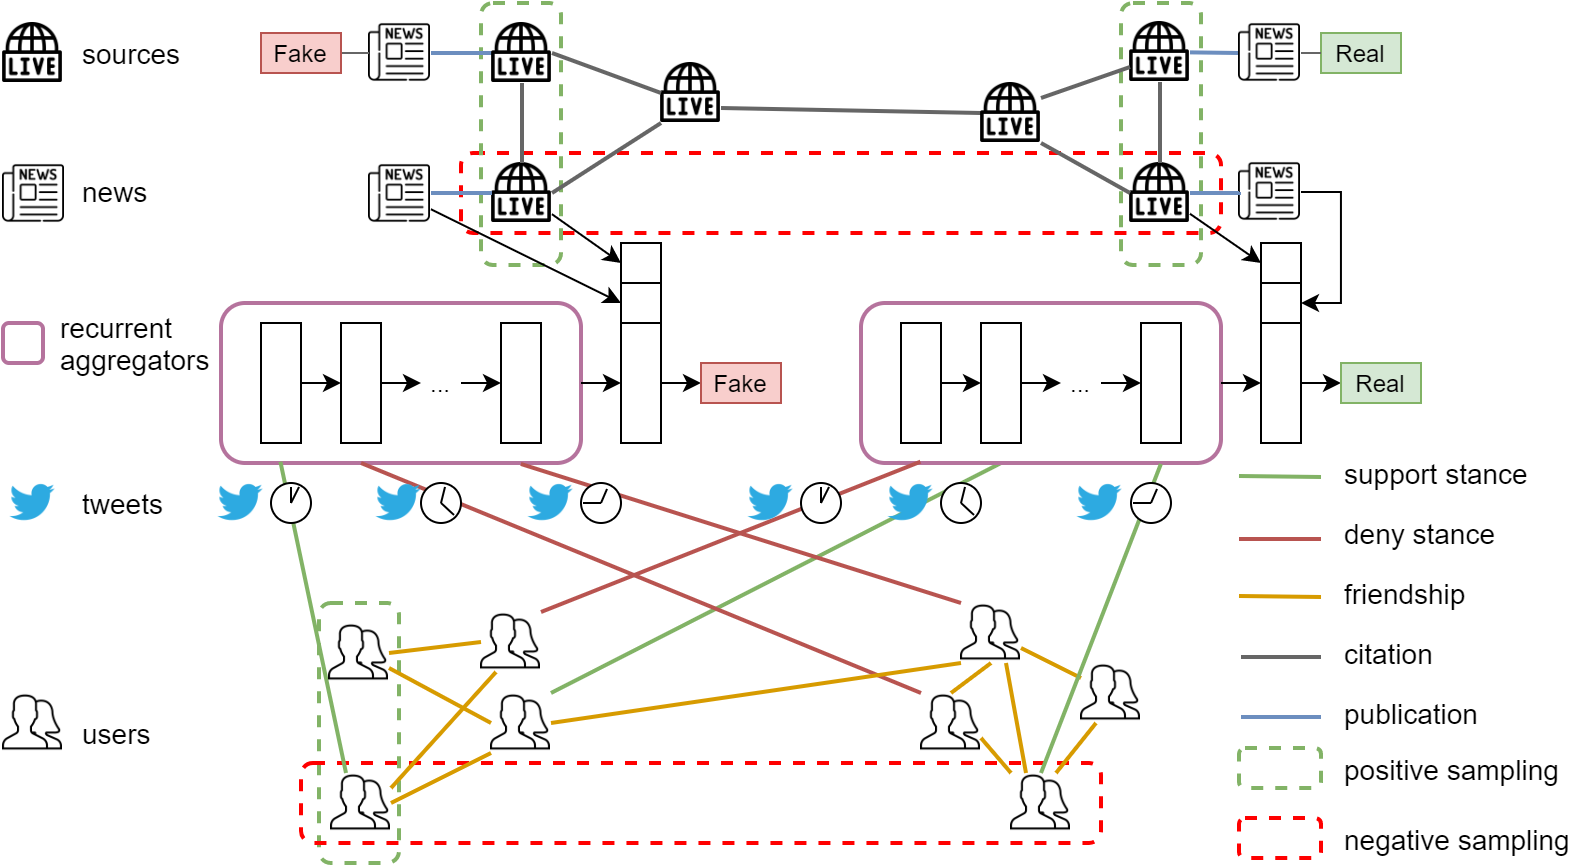
\includegraphics[scale=0.235]{fang.png}
\caption{Overview of the FANG framework.}
\label{fig:fang_overview}
\end{figure*}


\textbf{Stance Detection.} The task of obtaining a viewpoint for a piece of text with respect to another piece of text is known as \textit{stance detection}. 
In the context of fake news detection, we are interested in the stance of a user reply with respect to the title of a questionable news.
% Hoang: fixed
% Min: again BUG GLOBAL tweet vs. post.  Pick one term and stick with it.
In this work, we consider three stances \textit{support}, \textit{deny}, and \textit{report}. We classify a post as verbatim reporting of the news article if it matches the article title after cleaning the texts from emojis, punctuation, stop words, and URLs.
% Hoang: specify the preprocessing techniques to determine if a post is a verbatim report.
% Min: what's the threshold?
We train a stance detector to classify the remaining posts as 
% certain threshold. We train a stance detector to classify the remaining tweets as
\textit{supports} or \textit{denies}.
Popular stance detection datasets either do not explicitly describe the target text~\cite{derczynski-etal-2017-semeval}, have a limited number of targets~\cite{sobhani-etal-2017-dataset,mohammad-etal-2016-semeval}, or formulate the source/ target texts differently (as in the \emph{Fake News Challenge}).
%\footnote{\scriptsize{\url{http://www.fakenewschallenge.org/}}}). 

To address this difficulty, we constructed our own dataset for stance detection between posts and news containing 2,527 labeled source--target sentence pairs from 29 news events. For each event with a reference headline, the annotators were given a list of related headlines and posts. They labeled whether each related headline or post supports or denies the claim made by the reference headline. Aside from the \emph{reference headline--related headline} or the \emph{headline--related post} sentence pairs, we also make second-order inferences for \emph{related headline--related post} sentence pairs. 

If such a pair expressed a similar stance with respect to the reference headline, the inferred stance for the \emph{related headline--related post} would be \textit{support}, and it would be \textit{deny} otherwise.

Tables~\ref{table:stance_annotation} and~\ref{table:stance_statistics} show example annotations and statistics about the dataset. The inter-annotator agreement as evaluated using Cohen's Kappa score is 
% Min: probably not so signficant to 4 digits of precision.
% 0.7776, 
0.78, indicating a substantial agreement.

%Kaz: It would be better to briefly mention other approaches you compared with Roberta  
In order to choose the best stance classifier, we fine-tuned on our dataset various pre-trained large-scale Transformers~\cite{devlin2019bert,yang2019xlnet,liu2019roberta}. Roberta~\cite{liu2019roberta} turned out to work best, achieving \textit{Accuracy} of 0.8857, \textit{$F_1$ score} of 0.8379, \textit{Precision} of 0.8365, and \textit{Recall} of 0.8395, 
and thus we chose it for our stance classifier. The stance prediction of a user--article engagement $e$ is given as $stance(e)$. 



% We now detail our social context graph construction. We specify the selected features for each social entity (\textit{i.e}., $x_a$, $x_s$, $x_u$) and how we obtain the labels for each social interaction (\textit{i.e}., $x_e$).

\subsection{Factual News Graph (FANG) Framework}\label{sec:fang}

We next describe our Factual News Graph (FANG) learning framework on the social context graph described in Section~\ref{sec:graph_construction}. Figure~\ref{fig:fang_overview} shows an overview of FANG. 
% Social representation of each entities are optimized on the basis of positive and negative sampling. News articles have its sources, its engaged user tweets and their stance aggregated using a recurrent model to predict for the news factuality. 
% Hoang: shortened the nav paragraph without repetition
% Min: still repetitive.  Heard it many times already.  Try to eliminate more repetition.
% FANG's motivation is not only to improve the performance of contextual fake news detection, but also to improve the quality of representation learning. That is, 
While optimizing for the fake news detection objective, FANG also learns generalizable representations for the social entities. This is achieved by optimizing three concurrent losses: (\emph{i})~unsupervised \textit{Proximity Loss}, (\emph{ii})~self-supervised \textit{Stance Loss}, and (\emph{iii})~supervised \textit{Fake News Detection Loss}.

\textbf{GraphSage Representation Learning}. We first discuss how FANG derives the representation of each social entity. Previous representation learning frameworks such as Deep Walk~\cite{perozzi2014deepwalk} and node2vec~\cite{grover2016node2vec} compute a node embedding by sampling its neighborhood and then optimizing for the proximity loss, similarly to the way this is done in word2vec, but this time the neighborhood is defined by the graph structure. These methods use the neighborhood structure only, and they are suitable when the node auxiliary features are unavailable or incomplete, \emph{i.e.},~when optimizing for each entity's structural representation separately. Recently, a new model was proposed, GraphSage~\cite{Hamilton2017InductiveRL}, which overcomes this limitation by allowing auxiliary node features to be used jointly with proximity sampling as part of the representation learning. 

Let $GraphSage(.)$ be GraphSage's node encoding function. Thus, we now can obtain the structural representation $\boldsymbol{z}_u\in \mathbb{R}^d$ of node $u$ as $\boldsymbol{z}_u=GraphSage(u)$, where $d$ is the structural embedding dimension.

\textbf{Unsupervised Proximity Loss}. We derive the Proximity Loss from the hypothesis that closely connected social entities often behave similarly. It is motivated by the echo chamber phenomenon, where social entities tend to interact with other entities of common interest to reinforce and to promote their narrative. This echo chamber phenomenon encompasses inter-cited news media sources publishing news of similar content or factuality, as well as social friends expressing similar stance towards news article(s) of similar content. Therefore, FANG should assign such nearby entities to a set of
% Hoang: I meant close by, so proximal is a better suitable word
% Min: closed?  or close by?
% closed vectors 
proximal vectors
in the embedding space. We also hypothesize that loosely connected social entities often behave differently from our observation that social entities are highly polarized, especially in left--right politics~\cite{boxell2017internet}. Thus, FANG should enforce that the representations of these disparate entities be highly distinctive.

The social interactions that define the above characteristics the most are user--user friendship, source--source citation, and news--source publication. As these interactions are either between (a)~sources and news or (b)~between news, we divide the social context graph into two sub-graphs, namely \emph{news--source sub-graph} and \emph{user sub-graph}. 
Within each sub-graph $G$, we formulate the Proximity Loss function:
% Hoang: Agree, L_prox works better
% Min: how about just L_prox instead of L_proximity.  Fit your eq. better.
\begin{equation}\label{eq:proximity_loss}
    \mathcal{L}_{prox.} =  - \sum_{u\in G} \sum_{u_p\in P_u} log(\sigma(\boldsymbol{z}_u^\top \boldsymbol{z}_{u_p})) + Q \cdot \sum_{u_n\in N_u} log(\sigma(-\boldsymbol{z}_u^\top \boldsymbol{z}_{u_n})), 
\end{equation}
where $z_u\in \mathbb{R}^d$ is the representation of entity $u$, $P_u$ is the set of nearby nodes or \textit{positive set} of $u$, and $N_u$ is the set of disparate nodes or \textit{negative set} of $u$,
%Kaz: Rewrite the following sentence: 
%$P_u$ is obtained my fixed length Random Walk, while $N_u$ is obtained by negative sampling. 
$P_{u}$ is obtained using our fixed-length
% Hoang: fixed
% Min: why RW in caps?
random walk, and $N_{u}$ is derived via negative sampling. 

Each $u_n\in N_u$ is sampled with a discrete probability density function $\forall v\in G\setminus P_u, P(u_n=v) = \frac{\boldsymbol{x}_u^\top \boldsymbol{x}_v}{Z}$, where $\boldsymbol{x}_u$ and $\boldsymbol{x}_v$ are the feature vectors of entity $u$ and $v$, and $Z$ is the probabilistic normalization factor. In other words, we choose the negative samples of an entity $u$ based on the feature distance between $u$ and the candidate sample $v$ which is not in the positive samples. By minimizing the proximity loss defined by Equation~(\ref{eq:proximity_loss}), we effectively force the representations of closed entities to be similar and the representations of disparate entities to be distinct.

\textbf{Self-supervised Stance Loss}.
We also put forward an analogous hypothesis for the user--news interaction in terms of stance. If a user expresses a stance with respect to a news article, their respective representations should be proximal
% Hoang: I have changed to proximal
% Min: closed or close by? BUG, I can't parse this sentence
in the stance space. For each stance $c$, we first learn a user projection function $\alpha_c(u) = \mathbf{A_c} z_u$ and a news article projection function $\beta_c(a) = \mathbf{B_c} z_a$ that map a node representation of $\mathbb{R}^d$ to representation in stance $c$ space of $\mathbb{R}^{d_c}$. Given a user $u$ and a news article $a$, we compute their similarity score in the stance $c$ space as $\alpha(u)^T \beta(a)$. If $u$ actually expresses stance $c$ towards $a$, we maximize this similarity score, and we minimize it otherwise. We interpret this as a stance classification objective, which can be optimized using the Stance Loss: 
% Min: very clear but a bit redundant.  Not a lot of information here in the formula because aside from the log() everything you already discussed.
\begin{equation}
    \mathcal{L}_{stance} = -\sum_{u,a,c} y_{u,a,c} log(f(u,a,c)), 
\end{equation}
where $f(u,a,c)$ is defined as $f(u,a,c) = \alpha_c(u)^T \beta_c(a)$ and
\[  y_{u,a,c} = \left\{
\begin{array}{ll}
      1 & \textrm{if } u \textrm{ expresses stance } c \textrm{ over } a \\
      0 & \textrm{otherwise}. \\
\end{array} 
\right. \]

\textbf{Supervised Fake News Loss}. We directly optimize for the main learning objective of fake news detection via the supervised Fake News Loss. This can be formulated as learning an aggregation function $F(a, s, U)$ that maps a questionable news $a$, its source $s$, and its engaged users $U$ to a real number in $[0, 1]$, indicating the probability of $a$ being trustworthy. As observed in Section~\ref{sec:introduction}, we hypothesize that there are distinctive temporal patterns between false and genuine information. Therefore, the aggregating model (\textit{i.e.},~the aggregator) has to be time-sensitive.
% Hoang: noticed with thanks
% Min: this section seems to verbose for what has become somewhat already standard.
% Min: can cut more here. SHORTEN
Recurrent Neural Networks fulfill this requirement: specifically, the Bidirectional LSTM (Bi-LSTM) can capture a long-term dependency in information sequence in both the forward and the backward directions~\cite{lstm1997hochreiter}. On top of the Bi-LSTM, we further incorporate an attention mechanism that focuses on essential engagement during the encoding process. Attention is not only expected to improve the model quality, but also its explanability~\cite{luong2015effective,vaswani2017attention}. By examining the model's attention, we know which social profiles influence the decision, leveraging human analytic capability. 

Our proposed LSTM input is a user--article engagement sequence $\{e_1, e_2,\cdots,e_{|U|}\}$. Let $meta(e_i)\in \mathbb{R}^l=(time(e_i),stance(e_i))$ be the concatenation $e_i$'s time since the news article publication and stance as a one-hot vector. Each engagement $e_i$ has its representation $\boldsymbol{x}_{e_i}= (\boldsymbol{z}_{U_i}, meta(e_i))$,
% Hoang: fixed
% Min BUG: time and stance are not mentioned in the equation.  please fix.  
% Min this section a bit redundant too.  Ok for submission but should be fixed in the camera ready.
where $\boldsymbol{z_{U_i}}=GraphSage(U_i)$. A Bi-LSTM encodes the engagement sequence and outputs two sequence of hidden states: (\emph{i})~a forward sequence,
$H^f={\boldsymbol{h}^f_1, \boldsymbol{h}^f_2,\ldots,
  \boldsymbol{h}^f_n}$ that starts from the beginning of the engagement sequence, and
(\emph{ii})~a backward sequence, $H^b={\boldsymbol{h}^b_1,
  \boldsymbol{h}^b_2,\ldots, \boldsymbol{h}^b_n}$ that starts from the
end of the engagement sequence. 
%For many sequence encoding tasks, knowing both past (left) and future (right) 
%END SHORTEN
% The states $\boldsymbol{h}^f_i$ and $\boldsymbol{h}^b_j$ in
% the forward and backward sequences are computed as follows:
% \begin{eqnarray}
%   \boldsymbol{h}^f_i=LSTM(\boldsymbol{h}^f_{i-1}, \boldsymbol{x_{e_i}}),
%   \hspace{1mm}\boldsymbol{h}^b_j=LSTM(\boldsymbol{h}^b_{j+1}, \boldsymbol{x_{e_j}}), \nonumber 
% \end{eqnarray}
% where $e$ is the number of encoder units, and $\boldsymbol{h}^f_i, \boldsymbol{h}^b_j\in \mathbb{R}^e$ are the $i^{th}$ and $j^{th}$ hidden state vector of the forward ($f$) and backward ($b$) sequence.

Let $w_i$ be the attention weight paid by our Bi-LSTM encoder to the forward ($\boldsymbol{h}^f_i$) and to the backward ($\boldsymbol{h}^b_i$) hidden states. This attention should be derived from the similarity of the hidden state and the news features, \textit{i.e.,}~how relevant the engaging users are to the discussed content, and the particular time and stance of the engagement. Therefore, we formulate the attention weight $w_i$ as:
\begin{equation}
    w_i = \frac{exp(\boldsymbol{z}_a \mathbf{M}_e  \boldsymbol{h}_i + meta(e_i) \mathbf{M}_m)}{\sum^n_{j=1}exp(\boldsymbol{z}_a \mathbf{M}_e \boldsymbol{h}_j + meta(e_j) \mathbf{M}_m)}.
\end{equation}

\noindent where $l$, $e$ are the meta dimension, and the encoder dimension, and $\mathbf{M}_e\in \mathbb{R}^{d\times e}$ and $\mathbf{M}_m\in \mathbb{R}^{l\times 1}$ are the optimizable projection matrices for engagement and meta features shared across all engagements. $w_i$ is then used to compute the forward and the backward weighted feature vectors as follows:
\begin{eqnarray}\label{eq:w_sum}
  \boldsymbol{h}^f=\sum^n_i w_i \boldsymbol{h}^f_i, 
  \quad\boldsymbol{h}^b=\sum^n_i w_i \boldsymbol{h}^b_i. 
\end{eqnarray}

Finally, we concatenate the forward and backward vectors to obtain a single representation engagement $\boldsymbol{r}_a\in\mathbb{R}^{2e}$ for article $a$.

To predict whether article $a$ is false, we use a combination of its structural representation $\boldsymbol{z}_a$, its engagement representation $\boldsymbol{r}_a$, and its source $s$'s structural representation $\boldsymbol{z}_s$. The article's contextual representation is obtained as a concatenation of all these representations; {\it i.e.}, $\boldsymbol{v}_a = (\boldsymbol{z}_a, \boldsymbol{r}_a, \boldsymbol{z}_s)$. This contextual representation is then input into a fully connected layer whose outputs are computed as $o_a = \mathbf{W}\boldsymbol{v}_a+b$ where $\boldsymbol{W}\in \mathbb{R}^{(2d+2e)\times 1}$ and $b\in \mathbb{R}$ are the weights and the biases of the layer. The output value $o_a \in \mathbb{R}$
is finally passed through a sigmoid activation function $\sigma(\cdot)$, and trained using the cross-entropy Fake News Loss $\mathcal{L}_{news}$, defined as:   
\begin{equation}
    \mathcal{L}_{news}=\frac{1}{T}\sum_a\{{y}_{a} \cdot log(\sigma({o}_{a}))+(1-{y}_{a})\cdot log(1-\sigma({o}_{a}))\}, 
\end{equation}
where $y_{a}=0$ if $a$ is a fake article and $1$ otherwise.

\textbf{End-to-end Total Loss}. We define the final, Total Loss 
%as the sum of 
by linearly combining these three component losses.  This loss function is differentiable, and it is thus trainable using gradient descent.

\begin{equation}
    \mathcal{L}_{total} = \mathcal{L}_{prox.} + \mathcal{L}_{stance} + \mathcal{L}_{news}. 
\end{equation}


\section{Experiments}

% \subsection{Data}
% Hoang: title changed accordingly
% \todo{Preslav: I suggest you call this subsection ``Data'', and you have 1. a paragraph about the pre-existing datasets you use, and 2. about any new datasets you have or any way you augment the pre-existing datasets.}

We conducted our experiments on a Twitter dataset collected by related~work in rumor classification~\cite{ma2016detecting} and fake news detection~\cite{shu2018fakenewsnet}. For each article, we collect its source, list of engaged users, and their tweets if they are not already available in the previous dataset.
% Hoang: clarify that we crawl additional data if they are not available
% \todo{Preslav: The use of passive here makes it unclear who collected it: you or it was in the dataset already?} 
This dataset also
% Hoang: mention the expansion of source data
% \todo{Preslav: Confusing. Is there a second ``our dataset''? Or is it still the other dataset? Or did you augment that other dataset with extra information?} 
includes Twitter profile description and the list of Twitter profiles each user follows. We expand the previous dataset by crawling additional data about media sources, including the content of their \emph{Homepage} and their \emph{About us} page, together with their frequently cited sources by collecting the hyperlink references from their \emph{Homepage}. The truth value of the articles, namely, whether they are fake or real news, are based on two fact-checking websites --- Snopes and Politifact. 
%Kaz: Need to anonymize for blind review. 
%We release the source code of FANG at~\url{https://github.com/nguyenvanhoang7398/GraphLearning}. 
We will release the source code of FANG and the stance detection fine-tuned dataset\footnote{https://github.com/XXX} if our work is accepted.
Table~\ref{table:dataset_statistics} shows some statistics about our dataset. 

\subsection{Fake News Detection Results}\label{sec:macroscopic}
We benchmark the performance of FANG on fake news detection against several competitive models: (\emph{i})~a content-only model, (\emph{ii})~a Euclidean contextual model, and (\emph{iii})~another graph learning model. 
In order to compare our FANG with the content-only model, 
we use a Support Vector Machine model on TF-IDF feature vectors constructed from the news content (see Section~\ref{sec:graph_construction}). 
%In addition, to compare 
We also compare our approach to a current Euclidean model,  
%we choose 
% Min: 
CSI~\cite{ruchansky2017csi}, a fundamental yet effective recurrent encoder that aggregates the user features, the news content, and the user--news engagements. We reimplemented the CSI with source features by concatenating the overall score for the users and the article representation with our formulated source description to obtain
% Hoang: This is the name of a module in CSI's original paper
% Min: what is the Integrated module?  Not mentioned previously?
the result vector for CSI's Integrated module mentioned in the original paper. Lastly, we compare against the GCN graph learning framework~\cite{kipf2016semi}. First, we represent each of $k$ social interactions in a separated adjacency matrix. We then concatenate GCN's output on $k$ adjacency matrices as the final representation of each node, before passing the representation through a linear layer for classification.
% To keep consistency with the original work, we define $X\in \mathbb{R}^{N\times d_1}$ to be the input node feature matrix where $X^{(i)}\in \mathbb{R}^{d_1}$ is the feature vector of $i^{th}$ social actor defined in Section~\ref{sec:graph_construction}. Let $d_l$ be the size of any node hidden representation obtained at the $l^{th}$ layer of GCN. We define the convolution operation in our graph consisting of multi-label edges as follows: 
% \begin{equation}
%     H_{l+1} = \parallel^{K}_{k=1}(\tilde{D}^{-\frac{1}{2}}\tilde{M}_k\tilde{D}^{-\frac{1}{2}}H_l\Theta_l), 
% \end{equation}
% where $H_l\in \mathbb{R}^{N\times d_l}$ is the hidden representation matrix of social actors at $l^{th}$ layer, $\parallel$ is the concatenation operation, $K$ is the number of relations, $\Theta\in\mathbb{R}^{d_l\times d_{l+1}}$ is the matrix of optimizable weights at $l^{th}$ layer, and $\tilde{D}^{-\frac{1}{2}}\tilde{M}_k\tilde{D}^{-\frac{1}{2}}$ is the computation to obtain normalized graph Laplacian matrix. Notice that $H_1=X$ is the input feature matrix. After $L$ layers, we obtain the output vector as the final hidden representation of each article $a$, or $\boldsymbol{o_a}=H^{(\bar{a})}_L$ where $\bar{a}$ is the index of $a$. $\boldsymbol{o_a}$ is passed through a softmax activation function $\sigma$, and all learnable weights are trained using cross-entropy loss $\mathcal{L}$ defined as follows: 
% \begin{equation}\label{eq:overall_loss}
%     \mathcal{L}=\frac{1}{|A_c|}\sum^{A_c}_{a}\boldsymbol{y}_{a} \cdot log(\sigma(\boldsymbol{o}_{a}))+(1-\boldsymbol{y}_{a})\cdot log(1-\sigma(\boldsymbol{o}_{a}))
% \end{equation}

% Min: maybe you need to indicate what the ``i-'' indicates?  You weren't explicit. 
We also verified the importance of modeling temporality by experimenting on two variants for both CSI and FANG: (\emph{i})~temporal insensitive i-CSI and i-FANG without $time(e)$ in the engagement $e$'s representation $\boldsymbol{x}_{e}$, and (\emph{ii})~temporal sensitive CSI and FANG with $time(e)$. 

%The macroscopic results are presented in Table~\ref{table:macroscopic}. 

%Kaz: Rewrite
%All context-aware models, namely i-CSI, CSI, GCN, i-FANG, 
Table~\ref{table:macroscopic} shows the macroscopic results. 
For evaluation, we use $F_1$ score as standard, which is the harmonic mean of Precision and Recall. 
All context-aware models (\textit{i.e.},~i-CSI, CSI, GCN, and i-FANG) and FANG improve over the context-unaware baseline by .0744 absolute
% Hoang: convert all the improvement margin to absolute decimals instead of percentage.
% \todo{Preslav: I am confused why you talk here about \%. Table 7 gives the results in numbers in [0;1]. Is this relative or absolute improvement that you give in \%?} 
with i-CSI and by .2734 absolute with FANG in terms of $F_1$. This demonstrates that considering social context is helpful for fake news detection. %Secondly, 
We further observe that both time-sensitive CSI and FANG improve over their time-insensitive variants, i-CSI and i-FANG by .0526 and .063 respectively. These results demonstrate the importance of modeling the temporality of news spreading. Finally, two graph-based models, i-FANG and GCN are consistently better than the Euclidean CSI by .0561 and .136, respectively: this demonstrates the effectiveness of our social graph representation described in Section~\ref{sec:graph_construction}. Overall, we can see that FANG outperforms the other context-aware, temporally-aware, and graph-based models.
% Min: how about 
%Kaz: I think the following phrase is no need as it has already described above.  
%confirming the improvement of FANG in fake news detection.
%Kaz: Better to put Table 6 here 
\begin{table}[tb]
    \centering
    \small
    \caption{Statistics about our dataset.}
    \begin{tabular}{l@{}rlrlr} 
    \toprule
        Fake & 150 & Citations / source & 5.1 &  Support / news & 99.1 \\
        Real & 151 & Publications / source & 1.5 & Deny / news & 13.4 \\
        Sources & 199 & Friendship / user & 85.8 & Report / news & 70.3 \\
        Users & 85,394 & Engagements / news & 182.8 & & \\ 
        \bottomrule
    \end{tabular}
    \label{table:dataset_statistics}
\end{table}

\begin{table}[tb]
    \centering
    \small
    \caption{Comparison between FANG and baseline models in fake news detection evaluated with $F_1$ score.}
    \begin{tabular}{lcccc} 
    \toprule
        \bf Models & \bf Contextual & \bf Temporal & \bf Graphical & \bf $F_1$ score \\ 
    \midrule
        Feature SVM & & & & 0.6785 \\
        i-CSI & \checkmark & & &  0.7529 \\
        CSI & \checkmark & \checkmark & & 0.8055 \\ 
        GCN & \checkmark & & \checkmark & 0.8090 \\
        i-FANG & \checkmark & & \checkmark & 0.8889 \\ \hline
        \textbf{FANG} & \checkmark & \checkmark & \checkmark & 0.9519 \\ 
        \bottomrule
    \end{tabular}
    \label{table:macroscopic}
\end{table}


\section{Discussion}\label{sec:discussion}

% \todo{Preslav: Again ``ratioonale'' is the wrong term.}
We want to answer the following research questions (RQs) to better understand FANG's performance under different scenarios: 
\begin{itemize}
    \item RQ1: Does FANG work well with limited training data?
    \item RQ2: Does FANG differentiate fake and real news based on their contrastive engagement temporality?
    % Hoang: rephrase this RQ
    % \todo{Preslav: I do not understand this question. ``Rationale'' is ``a set of reasons or a logical basis for a course of action or belief'', i.e., it is the motivation. I do not see how your motivation can be a RQ. This needs to be rephrased.}
    \item RQ3: How effective is FANG's representation learning?
\end{itemize}

\subsection{Limited Training Data (RQ1)}

To address RQ1, we conduct the experiments described in Section~\ref{sec:macroscopic} given various training data sizes. These experiments confirm our model's consistent absolute performance and relative improvement over the baseline models under both limited and sufficient data.
% Hoang: I think it can be easier to read both the absolute results (in table) and relative results (in plot) 
% Min: why do you need both forms?
The experimental results are shown in Table~\ref{table:limited_data} and are further visualized in Figure~\ref{fig:limited_and_attention} (left).
% Hoang: I will develop this point in future experiments
% Min: is the variance of FANG better than in the other cases?  Can you use that as a means to argue for its effectiveness?
% Min: do you need to describe more about how you do the splits? Are they temporally correctly split? i.e., no training data comes from the future?
We can see that FANG consistently outperforms two baselines at all given training sizes of 10\%, 30\%, 50\%, 70\%, and 90\% of the data. Among the graph-based models, GCN's performance drops by 24.31\% from 0.809 in $F_1@0.9$ to 0.6123 in $F_1@0.1$, while FANG's performance drops by 13.07\% from 0.9519 in $F_1@0.9$ to 0.8274 in $F_1@0.1$. We also observe that CSI's performance drops least by only 7.76\% from 0.8055 in $F_1@0.9$ to 0.743 in $F_1@0.1$. 
% Hoang: omit this conjecture
% Min: BUG this is conjecture without evidence.  You need some analysis to show this.
% This high generalization can be explained by the simplicity of Euclidean models as they are built upon the ``independent and identically distributed'' assumption for random variables. 
Overall, the experimental results highlight our model's effectiveness even at low training availability compared to its GNN and Euclidean counterparts, which confirms RQ1. 

\subsection{Engagement Temporality Study (RQ2)} 

To address RQ2 and verify whether our model makes its decision based on the distinctive temporal patterns between fake and real news, we examine FANG's attention mechanism. We accumulate the attention weights produced by FANG within each time window and compare them across time windows. Figure~\ref{fig:limited_and_attention} (right) shows the attention distribution over time with respect to fake and real news.
\begin{table}[t]
    \centering
    \small
    \caption{Comparison of FANG against baselines ($F_1$ score) by varying the size of the training data. The last column on $F_1@0.9$ is identical to Table~\ref{table:macroscopic}.}
    \begin{tabular}{l  l l l l l} 
    \toprule
        \bf Systems & \bf $F_1@0.1$ & \bf $F_1@0.3$ & \bf $F_1@0.5$ & \bf $F_1@0.7$ & \bf $F_1@0.9$ \\
    \midrule
        CSI & 0.743  & 0.7443  & 0.6851 & 0.7546 & 0.8055 \\
        GCN & 0.6123 & 0.6866  & 0.6407 & 0.6523 & 0.8090 \\ \hline
        FANG & 0.8274 & 0.8366 & 0.8010 & 0.8218 & 0.9519 \\ 
    \bottomrule
    \end{tabular}
    \label{table:limited_data}
\end{table}

\begin{figure}[t]
\centering
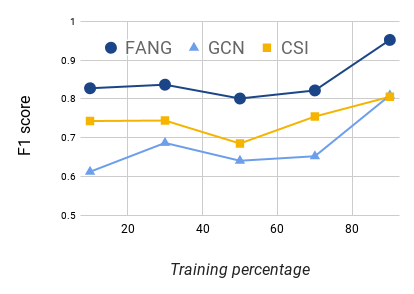
\includegraphics[scale=0.25]{chart.png}
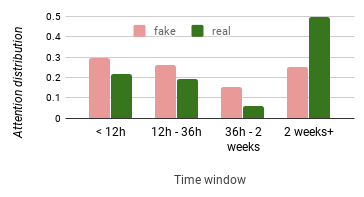
\includegraphics[scale=0.35]{fang_attention.png}
\caption{FANG's performance against baselines ($F_1$ score) for varying training data sizes (left), and attention distribution across time windows for fake vs. real news (right).}
\label{fig:limited_and_attention}
\end{figure}

We observe that FANG pays almost 60\% of its attention to the user engagement that occurred in the first 36 hours (approximately 30\% on the first 12 hours and 26\% on the 12 to 36 hours) after a news article has been published to decide whether it is fake. Its attention then sharply decreases to 15\% for the time window of 36 hours to two weeks after publication, and then to approximately 25\% from the second week onward. On the other hand, for real news, FANG maintains approximately 40\% of its attention on the first 36 hours, but places much more attention of 50\% after two weeks since publication. 

Our model's characteristic is consistent with the general observation that the appalling nature of fake news generates the most engagements within a short time after its publication. Therefore, it is reasonable that the model places emphasis on these crucial engagements. On the other hand, genuine news attracts fewer engagements, but it is circulated for a longer period of time, which explains FANG's persistent attention even after two weeks after publication. Overall, the temporality study highlights the transparency of our model's decision, largely thanks to the incorporated attention mechanism. 
% Min: omit sentence, vacuous
% We also analyze how FANG's decisions arise from the different spreading patterns of fake and real news, which confirms RQ2.
% Hoang: noticed with thanks. We can examine instantaneous fake news detection
% Min: future work, what about cases where fake news needs to be detected and declared earlier, at less than two weeks old?  Is FANG better than other systems for doing that?

\subsection{Representation Learning (RQ3)}

Our central claim is to improve the quality of representation with FANG, and we verify it in intrinsic and extrinsic evaluations. 

In the intrinsic evaluation, we verify how generalizable the minimally supervised news representations are in the fake news detection task. We first optimize both GCN and FANG on 10\% of the training data to obtain all news representations. We then cluster these representations using Mean Shift (MS)~\cite{Comaniciu2002meanshift}, an unsupervised clustering algorithm, and we measure the homogeneity score --- the extent to which clusters contain a single class. 
The higher the homogeneity score, the more likely the news articles of the same factuality label (\textit{i.e.},~fake or real) are close to each other, and thus the higher the quality of the representation. 
We visualize the representations obtained from two approaches with factuality labels and MS clustering labels in Figure~\ref{fig:fang_rep}.

In the extrinsic evaluation, we verify how generalizable the sufficiently supervised source representations are for the extrinsic source factuality task. We first train FANG on 90\% of the training data to obtain all source $s$'s representation as $z_s=GraphSage(s)$, and then we obtain source $s$'s total representation $r_s$ as follows: 
\begin{equation}
    v_s=(z_s,x_s,\sum_{a\in publish(s)}x_a), 
\end{equation}
where $x_s$, $publish(s)$, and $x_a$ denote source $s$'s content representation, the list of all articles published by $s$, 
and  their content representations, respectively. 

%Kaz: Moved to Figs 5 and 6 so that they are at the top of the page
\begin{figure}[t]
\centering
\fbox{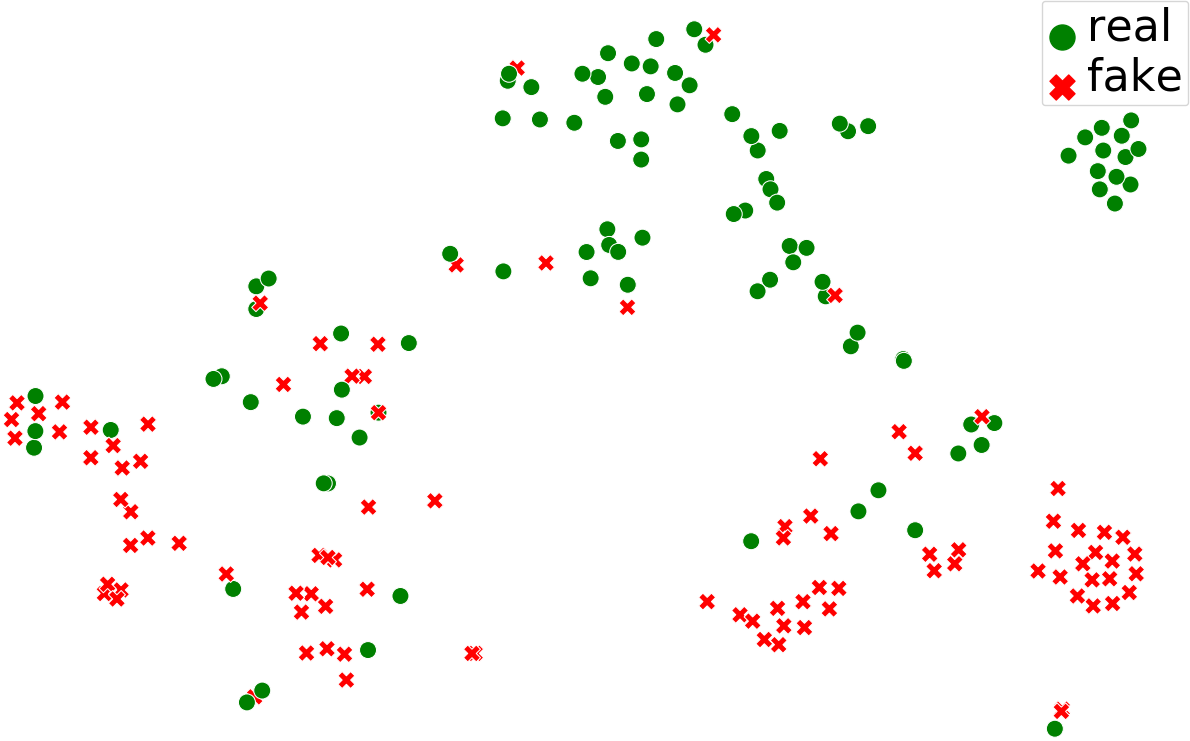
\includegraphics[scale=0.089]{fang_tsne.png}}
\fbox{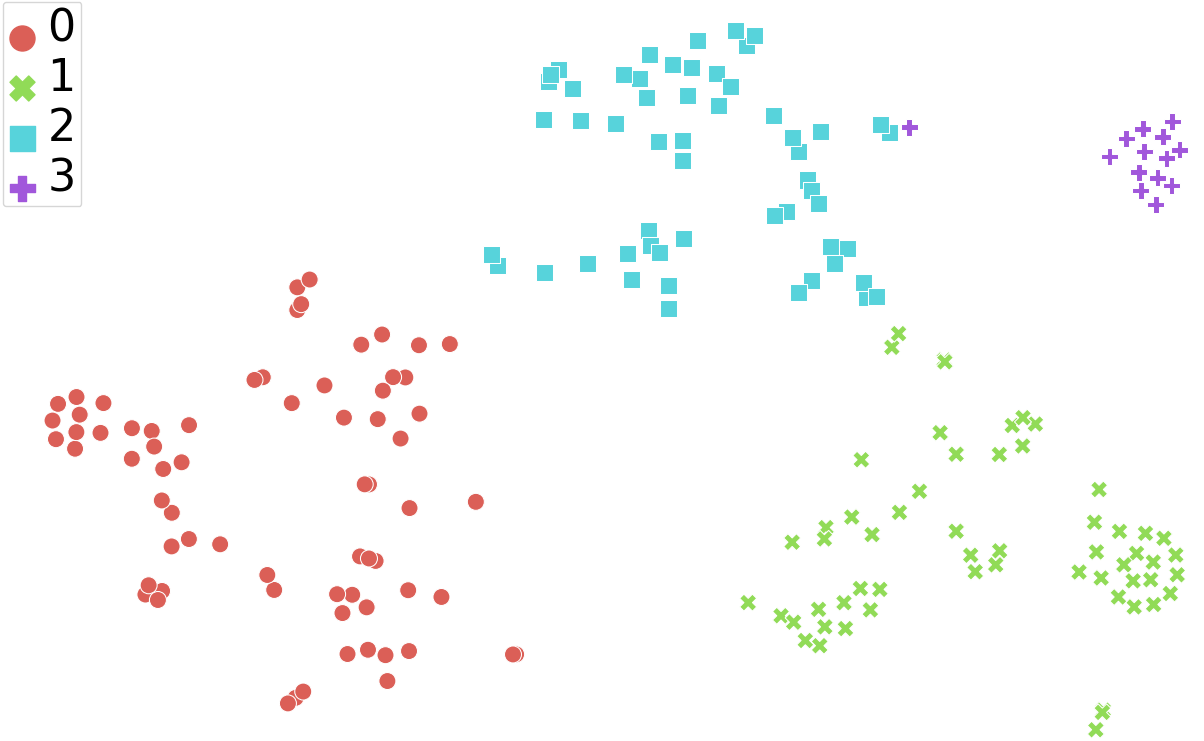
\includegraphics[scale=0.089]{fang_clusters.png}}\\
\fbox{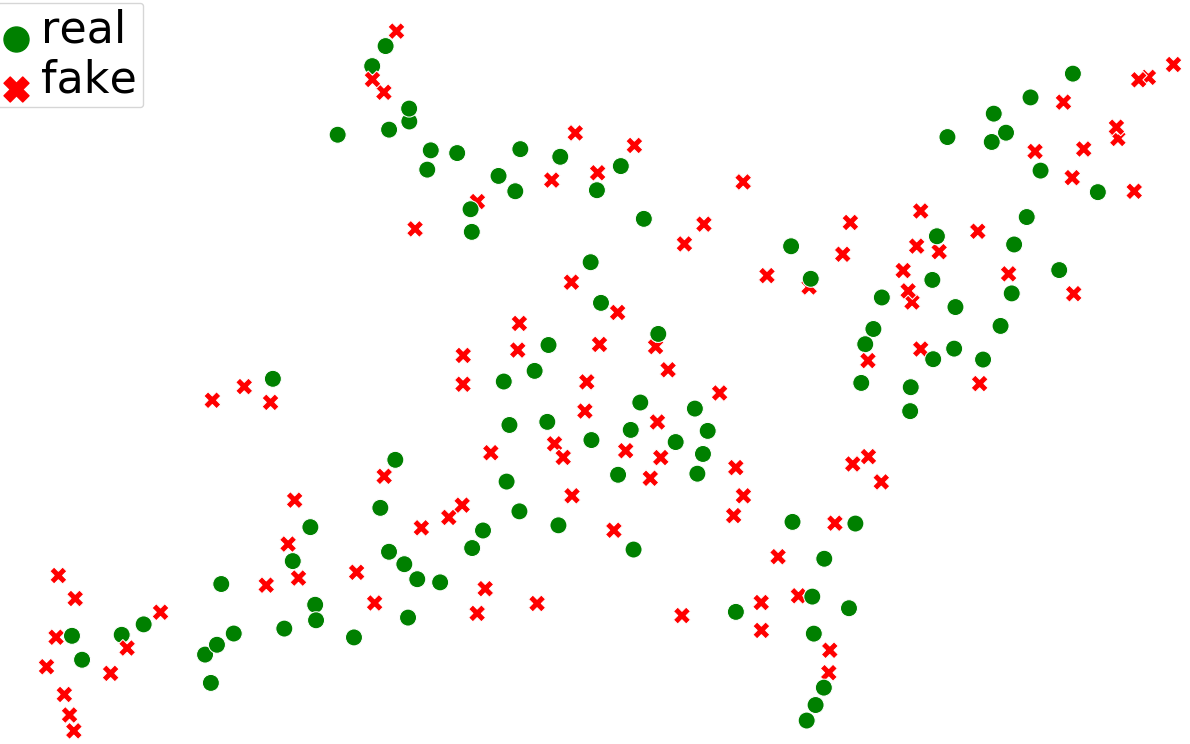
\includegraphics[scale=0.089]{gcn_tsne.png}}
\fbox{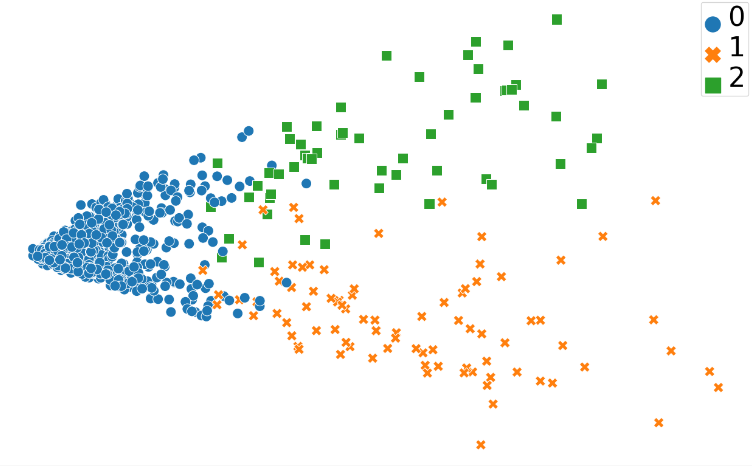
\includegraphics[scale=0.09]{gcn_clusters.png}}\\
\caption{2D t-SNE plot of FANG's representations with factuality news labels (top left) and MS clustering labels (top right), and GCN's news representations with factuality news labels (bottom left) and MS clustering labels (bottom right).}
\label{fig:fang_rep}
\end{figure}

We propose two baseline representations that do not consider source $s$ content, $v^{\prime}_s=(z_s,x_s)$. Finally, we train two separate SVM models for $v_s$ and $v^{\prime}_s$ on the source factuality dataset, consisting of 39 sources of high factuality and 39 sources of low factuality. 
%Kaz: Please specify the name of the Web site. 
The source factuality labels are obtained from Media Bias/Fact Check\footnote{\url{https://mediabiasfactcheck.com/}} and PolitiFact.

% \begin{table}[ht]
%     \centering
%     \small
%     \caption{Some statistics of our source factuality dataset.}
%     \begin{tabular}{l | l l} \hline
%          & High factuality & Low factuality \\ \hline
%         Train & 17 & 21  \\
%         Test & 22 & 18 \\ \hline
%     \end{tabular}
%     \label{table:source_dataset}
% \end{table}

% \begin{table}[ht]
%     \centering
%     \small
%     \caption{Performance of our proposed model versus baseline on source factuality classification in terms of $F_1$ score.}
%     \begin{tabular}{c | c | c} \hline
%         Systems & Context-aware & $F_1$ score \\ \hline
%         Baseline &  & 0.5535 \\
%         Proposed & \checkmark & 0.6350 \\ \hline
%     \end{tabular}
%     \label{table:source_results}
% \end{table}

\begin{figure*}[t]
\centering
\fbox{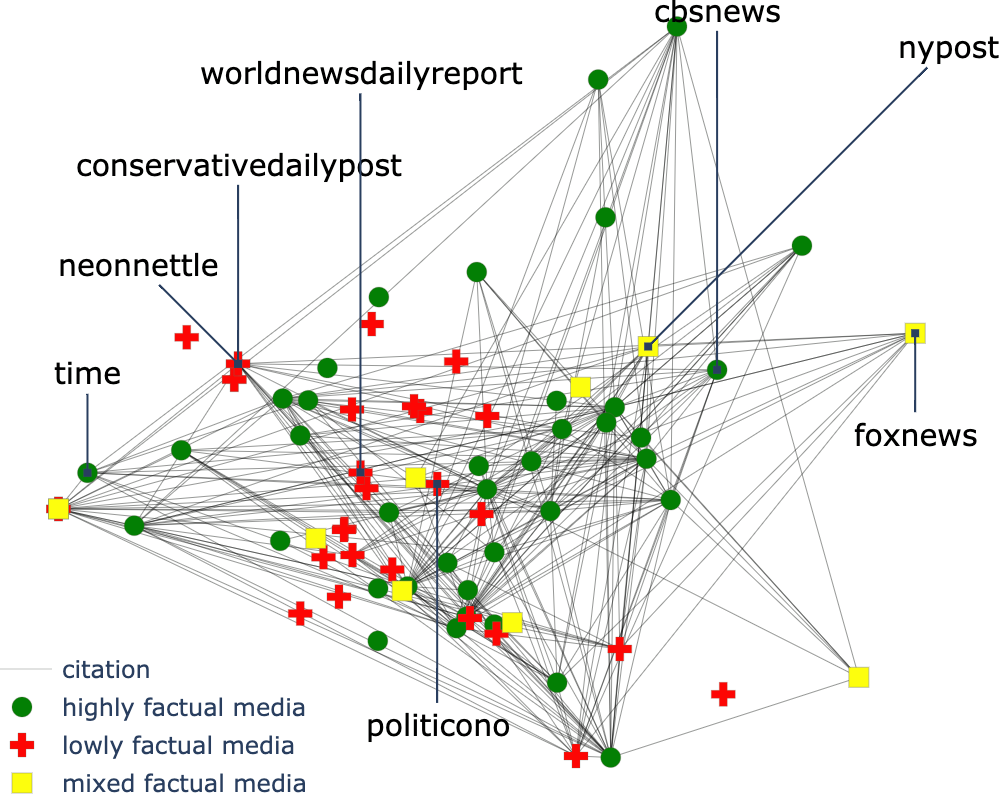
\includegraphics[width=6cm, height=5.1cm]{source_origin.png}}
\fbox{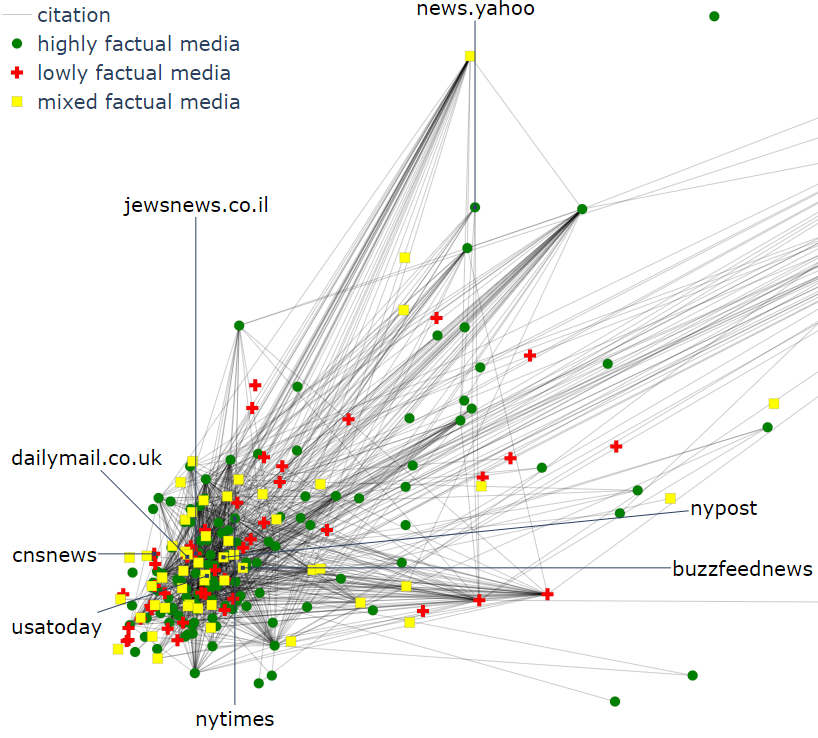
\includegraphics[width=4cm, height=5.1cm]{source_gcn.png}}
\fbox{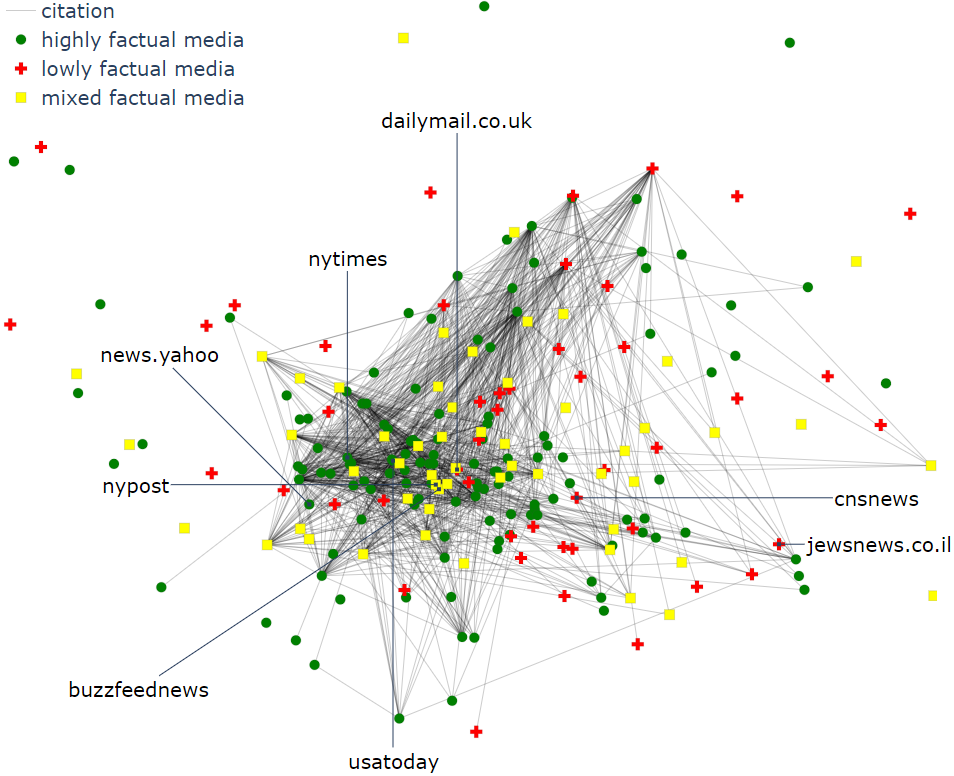
\includegraphics[width=6.85cm, height=5.1cm]{source_fang.png}}\\
\caption{Plots for source representations using textual features (left), GCN (middle), and FANG (right) with factuality labels.}
\label{fig:source_rep}
\end{figure*}

For instrinsic evaluation, the t-SNE plot of labeled FANG's (Figure~\ref{fig:fang_rep}'s top left) representation shows a moderate collocation within the two groups of fake and real news, while the t-SNE plot of labeled GCN's representation (Figure~\ref{fig:fang_rep}'s bottom left) shows no significant collocation within any group of fake or real news. Quantitatively, FANG's MS clusters as shown in (Figure~\ref{fig:fang_rep}'s right) obtain a homogeneity score of 0.3027 based on news factuality labels, compared to 0.0122 homogeneity score obtained for the GCN MS clusters. This intrinsic evaluation shows FANG's strong representation closeness within both fake and real news groups, indicating that FANG yields improved representation learning over another fully supervised graph neural framework. 

%Kaz: Moved figures at the top 
\begin{figure}[t]
\centering
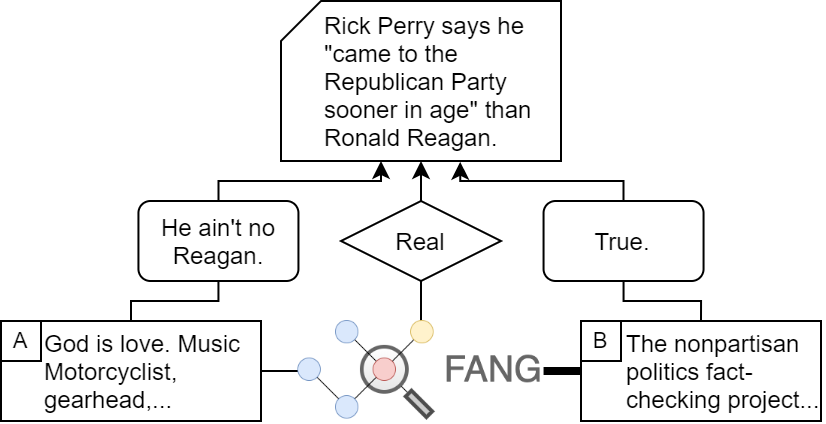
\includegraphics[scale=0.28]{micro1_chart.png}
\caption{A test example explaining FANG's decision.}
\label{fig:micro_1}
\end{figure}

For extrinsic evaluation on downstream source factuality classification, our context-aware model achieves an $F_1$ score of  $0.6350$ compared to $0.5535$ for the baseline. We further examine FANG's representations for sources to explain this .0815 absolute improvement. Figure~\ref{fig:source_rep} shows the source representations obtained from the textual features, GCN, and FANG with their factuality labels \textit{i.e.},~high, low, mixed, and citation relationship. In the left sub-figure, we can observe that the textual features are insufficient to differentiate the factuality of media, as a fake news spreading site such as \textit{politicono} mimics the original website  -- \textit{politico}'s content. However, the citation between the fake website and other highly factual sites is not as high, and was effectively utilized by the two graph learning frameworks -- GCN and especially FANG. Yet, GCN poorly differentiates low-factuality sites with higher citation like \textit{neonnettle} or \textit{conservativedailypost} from highly factual sites. FANG, with a greater emphasis on representation learning, represents these sources more distinguishably. 

We also spot a limitation where all three models failed to differentiate mixed factual media \textit{i.e.},~\textit{foxnews}, \textit{nypost} which do not always report factual news but have high citation with other highly factual sources.
Overall, the results from intrinsic and extrinsic evaluation as well as the observations confirm RQ3 on the improvement of FANG's representation learning.


\subsection{Microscopic Analysis}

It's also helpful to validate our model's prediction by examining specific test examples.  In the first example (Figure~\ref{fig:micro_1}),
%a news titled ``Ricky Perry says he came to the Republican Party sooner in age than Ronald Reagan.'' 
we see that FANG pays most of its attention to a tweet by \textit{user B}. This can be explained by B's Twitter profile description of a fact-checking organization, indicating a high reliability. In contrast, a denying tweet from \textit{user A} is not paid as much attention due to the insignificant description of its author's profile. Our model bases its prediction of the news article being true thanks to the support stance of the fact-checker, which is indeed the correct label.

\begin{figure}[t]
\centering
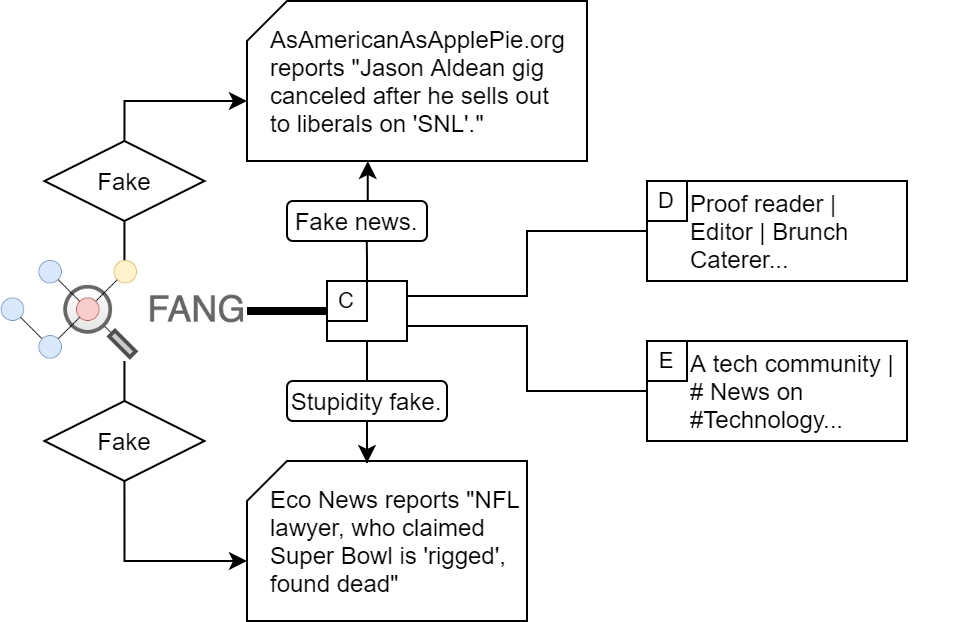
\includegraphics[scale=0.25]{micro2_chart.png}
\caption{Another test example explaining FANG's decision.}
\label{fig:micro_2}
\end{figure}

In the second example (Figure~\ref{fig:micro_2}), 
% a news titled  ``Jason  Aldean gig canceled after he sells out to liberals on "SNL"'', 
FANG pays most attention to a tweet by \textit{user C}. Although this profile does not provide any description, it has a record of correctly denying the fake news about the dead NFL lawyer. Furthermore, the profiles that follow Twitter user C, namely \textit{user D} and \textit{user E}, have credible description of a tech community and a proof reader. This explains why our model bases its prediction of the news being fake thanks to the reliable denial, again the correct label.

\subsection{Limitations}
We note that entity and interaction features are constructed before passing to FANG. Errors from upstream tasks, such as textual encoding or stance detection, can be propagated and can affect FANG's downstream performance. 

Future work can address this in an end-to-end framework where advanced textual encoding~\cite{devlin2019bert} and stance detection can be jointly optimized under the fake news detection objective. 

Another limitation is that the dataset for contextual fake news detection can quickly become obsolete as hyperlinks and social media traces at the time of publication might no longer be retrievable.

\section{Conclusion and Future Work}

We have demonstrated the importance of modeling the social context for the task of fake news detection. We further proposed FANG, a graph learning framework that enhances representation quality by capturing the rich social interactions between users, articles, and media, thereby improving both fake news detection and source factuality prediction. 
We have demonstrated the efficiency of FANG with limited training data and its capability of capturing distinctive temporal patterns between fake and real news with a highly explainable attention mechanism. 

In future work, we plan more analysis of the representations of social users. We further want to try multi-task learning for jointly addressing the tasks of fake news detection, source factuality prediction, and echo chamber discovery.

% \begin{acks}
% To Robert, for the bagels and explaining CMYK and color spaces.
% \end{acks}


\bibliographystyle{ACM-Reference-Format}
\bibliography{sample-base}

\appendix

\end{document}
\endinput
%%
%% End of file `sample-authordraft.tex'.
